%Editor: We have provided a PDF that shows the tracked changes in your file as in a Word document. This method makes it easier for you to match the edited file with your original file and make any necessary edits to your file in your LaTeX program. Please let us know if you require further assistance.
%%%%%%%%%%%%%%%%%%%%%%%%%%%%%%%%%%%%%%%%%%%%%%%%%%%%%%%%%%%%%%%%%%%%%%%%%%%%%%%%%%%%%%%%%%%%%%%%%%%%%%%%%%%%%%%%%%%%%%%%%%%%%%%%%%%%%%%%%%%%%%%%%%%%%%%%%%%
% This is just an example/guide for you to refer to when submitting manuscripts to Frontiers, it is not mandatory to use Frontiers .cls files nor frontiers.tex  %
% This will only generate the Manuscript, the final article will be typeset by Frontiers after acceptance.   
%                                              %
%                                                                                                                                                         %
% When submitting your files, remember to upload this *tex file, the pdf generated with it, the *bib file (if bibliography is not within the *tex) and all the figures.
%%%%%%%%%%%%%%%%%%%%%%%%%%%%%%%%%%%%%%%%%%%%%%%%%%%%%%%%%%%%%%%%%%%%%%%%%%%%%%%%%%%%%%%%%%%%%%%%%%%%%%%%%%%%%%%%%%%%%%%%%%%%%%%%%%%%%%%%%%%%%%%%%%%%%%%%%%%

%%% Version 3.4 Generated 2018/06/15 %%%
%%% You will need to have the following packages installed: datetime, fmtcount, etoolbox, fcprefix, which are normally inlcuded in WinEdt. %%%
%%% In http://www.ctan.org/ you can find the packages and how to install them, if necessary. %%%
%%%  NB logo1.jpg is required in the path in order to correctly compile front page header %%%

\documentclass[utf8]{FrontiersinHarvard} % for articles in journals using the Harvard Referencing Style (Author-Date), for Frontiers Reference Styles by Journal: https://zendesk.frontiersin.org/hc/en-us/articles/360017860337-Frontiers-Reference-Styles-by-Journal
%\documentclass[utf8]{FrontiersinVancouver} % for articles in journals using the Vancouver Reference Style (Numbered), for Frontiers Reference Styles by Journal: https://zendesk.frontiersin.org/hc/en-us/articles/360017860337-Frontiers-Reference-Styles-by-Journal
%\documentclass[utf8]{frontiersinFPHY_FAMS} % Vancouver Reference Style (Numbered) for articles in the journals "Frontiers in Physics" and "Frontiers in Applied Mathematics and Statistics" 

%\setcitestyle{square} % for articles in the journals "Frontiers in Physics" and "Frontiers in Applied Mathematics and Statistics" 
\usepackage{url,hyperref,lineno,microtype,subcaption}
\usepackage[onehalfspacing]{setspace}
\usepackage{caption}
\usepackage{graphicx}
\usepackage{float} 
%\usepackage{subfig} 
%\usepackage{subfloat}
\usepackage{inputenc}
\usepackage{amssymb}
\usepackage{amsmath}
\usepackage{amsfonts}
\usepackage{bbding}
\usepackage{xspace} 
\usepackage{latexsym}
\usepackage{color}
\usepackage{setspace}
\usepackage{multirow}
\usepackage{makecell}
\usepackage{soul}
\soulregister{\cite}7 % 注册\cite命令
\soulregister{\citep}7 % 注册\citep命令
\soulregister{\citet}7 % 注册\citet命令
\soulregister{\ref}7 % 注册\ref命令
\soulregister{\pageref}7 % 注册\pageref命令
\linenumbers



% Leave a blank line between paragraphs instead of using \\


\def\keyFont{\fontsize{8}{11}\helveticabold }
\def\firstAuthorLast{Sample {et~al.}} %use et al only if is more than 1 author
\def\Authors{Yang Guan\,$^{1}$, Xiaoyan Liu\,$^{1}$, Zhibin Yu\,$^{1,2,*}$, Yubo Wang\,$^{3}$, Xingyu Zheng\,$^{4}$, Shaoda Zhang\,$^{4*}$, Bing Zheng\,$^{1,2}$}
% Affiliations should be keyed to the author's name with superscript numbers and be listed as follows: Laboratory, Institute, Department, Organization, City, State abbreviation (USA, Canada, Australia), and Country (without detailed address information such as city zip codes or street names).
% If one of the authors has a change of address, list the new address below the correspondence details using a superscript symbol and use the same symbol to indicate the author in the author list.
\def\Address{$^{1}$Ocean University of China, Qingdao, China \\
$^{2}$Sanya Oceanographic Institution, Sanya, China \\ 
$^{3}$Xidian University, Xi’an, China \\
$^{4}$Cofoe Medical Technology Company Limited, Shenzhen, China }
% The Corresponding Author should be marked with an asterisk
% Provide the exact contact address (this time including street name and city zip code) and email of the corresponding author
\def\corrAuthor{Zhibin Yu, Shaoda Zhang}

\def\corrEmail{yuzhibin@ouc.edu.cn \\Alex@cofoe.com}




\begin{document}
\onecolumn
\firstpage{1}

\title[Running Title]{Fast Underwater Image Enhancement Based on a Generative Adversarial Framework}

\author[\firstAuthorLast ]{\Authors} %This field will be automatically populated
\address{} %This field will be automatically populated
\correspondance{} %This field will be automatically populated

\extraAuth{}% If there are more than 1 corresponding author, comment this line and uncomment the next one.
%\extraAuth{corresponding Author2 \\ Laboratory X2, Institute X2, Department X2, Organization X2, Street X2, City X2 , State XX2 (only USA, Canada and Australia), Zip Code2, X2 Country X2, email2@uni2.edu}


\maketitle


\begin{abstract}

%%% Leave the Abstract empty if your article does not require one, please see the Summary Table for full details.
Underwater image enhancement is a fundamental requirement in the field of underwater vision. Benefiting from the success of deep learning, underwater image enhancement has made remarkable progress. However, most deep learning-based enhancement methods are computationally expensive, which restricts their application in real-time \textit{large-size} underwater image processing. Furthermore, GAN-based methods tend to generate spatially inconsistent styles that decrease the enhanced image quality. To solve these problems, we propose a novel efficiency model based on a generative adversarial framework for \textit{large-size} underwater image enhancement, named FSpiral-GAN. We design our model with equal upsampling blocks (EUBs), equal downsampling blocks (EDBs) and lightweight residual channel attention blocks (RCABs), effectively simplifying the network structure and solving the spatial inconsistency problem. Enhancement experiments on a large number of real underwater datasets demonstrate the advanced performance and improved efficiency of our model.

\tiny
 \keyFont{ \section{Keywords:} Generative adversarial networks, efficiency, spatial inconsistency, underwater image enhancement, lightweight} %All article types: you may provide up to 8 keywords; at least 5 are mandatory.
\end{abstract}

\section{Introduction}

In recent years, underwater robots such as remotely operated vehicles (ROVs) have been widely used in important tasks such as deep-sea exploration~\citep{whitcomb2000advances}, marine species migration, coral reef monitoring~\citep{6385685} and the salvage of sunken ships. ROVs use \textit{large-size} (\textit{e.g.,} 960p ($1280\times960$) ~\citep{goodman2003development} underwater vision data to perform the above engineering tasks~\citep{2016Ship}. However, the absorption and scattering of underwater light cause problems such as low contrast, color deviation, and blurred details, seriously affecting the performance of further vision tasks such as exploration, intelligent analysis or subsea operations. Although there has been some progress in the study of underwater image enhancement~\citep{8460552}~\citep{9001231}~\citep{naik2021shallow}, these models can only process \textit{small-size} (\textit{e.g.} $256\times256$) images in real time, so designing a practical underwater enhancement model for real-time \textit{large-size} underwater image processing is still challenging.

Some early underwater image enhancement approaches, such as CLAHE~\citep{109340}, can provide a fast and real-time solution. However, these approaches always suffer from heavy color distortion and noise caused by scattering and absorption~\citep{lu2017underwater}. Due to the success of deep learning, data-driven approaches provide a potential solution for underwater image enhancement~\citep{naik2021shallow,2019Underwater1}. As one of the most popular areas of deep learning, GAN-based image-to-image (I2I) methods provide a general framework for underwater image enhancement~\citep{9001231}. However, most I2I-based methods suffer from the contradiction between image quality and processing speed, especially when the input image is large. A larger input image always leads to larger feature maps and greater computational complexity. Some researchers have indicated that the model parameters and processing time could be reduced by using knowledge distillation~\citep{ren2021online}. However, for underwater image enhancement tasks, reducing channels and layers is more likely to cause color shifting and distortion~\citep{2020Underwater}~\citep{guo2019underwater}~\citep{zhuang2021retinex}. Simultaneously improving underwater image quality and translation efficiency is challenging. zhang2022underwater

To alleviate this problem, FUnIE-GAN is used for upsampling and downsampling to reduce the feature map size and speed up the enhancement process. However, the channel efficiency is not considered in FUnIE-GAN, which makes this approach insufficient for handling the real-time \textit{large-size} underwater enhancement task. Even a low-cost underwater camera can provide a \textit{large-size} video flow (e.g., 720p, 960p or 1080p). These deep learning-based models are unable to be deployed on ROVs due to their high computation costs, which hinder their further applications. In ShuffleNetv2~\citep{2018ShuffleNet}, when the input channels are equal to the output channels, the memory access cost (MAC) can be minimized to improve the model inference speed. Inspired by the ``equal channel strategy'' proposed in ShuffleNetv2, we propose an equal upsampling block (EUB) and equal downsampling block (EDB) to build a more efficient underwater image enhancement model.

It has been shown that many GAN-based models can improve the perceptual quality of underwater images as well as their contrast and color saturation~\citep{2020Underwater}~\citep{9001231}. However, GAN-based models can also generate spatially inconsistent styles and introduce artifacts~\citep{2021LAFFNet}~\citep{wang2021uiec}~\citep{8917818}. Based on experiments, we found that a lightweight GAN-based model is more likely to lead to spatial inconsistency due to its limited layer channels. To alleviate this problem without excessively increasing the parameters, we include residual channel attention blocks (RCABs). 

To improve the efficiency of the model while maintaining the quality of the enhanced images, we propose an end-to-end, fast and efficient framework for \textit{large-size} underwater enhancement tasks. Our generator is a lightweight encoder and decoder network with equal upsampling blocks (EUBs) and equal downsampling blocks (EDBs). In addition, we introduce a lightweight RCAB in the generator to solve the problem of spatial inconsistency, further improving the visual quality of the enhanced images. Our contributions are summarized as follows:
\begin{itemize}
\item We propose an efficient underwater image enhancement model based on a generative adversarial network, namely, FSpiral-GAN, which can handle a 960p enhanced underwater image task at a running speed of 40 FPS with a GPU (Figure~\ref{fig:start picture}\textbf{B}).

\item 
We propose an equal upsampling block (EUB) and equal downsampling block (EDB) to improve the computational efficiency so that a real-time \textit{large-size} underwater image enhancement task can be handled by minimizing the MAC.


\item We propose a novel architecture that includes RCABs and follows the U-Net design principles in the field of underwater image enhancement. Experimental results show that our architecture can effectively solve the problem of spatial inconsistency, and the color transition of images generated by the proposed model is more continuous, without obvious boundaries.

\item We provide qualitative and quantitative comparisons with other advanced methods on real underwater datasets. Experimental results prove that the proposed model has fewer floating-point operations (FLOPs) and faster image processing speed than state-of-the-art models while maintaining generated images with good visual quality.
\end{itemize}

\section{Related Work}
\subsection{Traditional Underwater Image Enhancement Methods}
Traditional underwater image processing methods can be divided into model-free enhancement methods and physical model-based restoration methods. 

Model-free methods do not consider the degradation principle of underwater imaging and improve the sharpness of the image by adjusting its pixel value. Ancuti \textit{et al.}~\citep{2012Enhancing} proposed an algorithm based on a fusion strategy that enhances underwater images and videos by using multiscale fusion that combines contrast-enhanced images and color-corrected images. In addition, many researchers have focused on retinex-based methods to improve the quality of underwater images. Fu \textit{et al.}~\citep{2015A} proposed a retinex-based underwater image enhancement algorithm, which includes color correction, layer decomposition, and contrast enhancement. By using bilateral and trilateral filtering in the three channels of an image in the CIELAB color space, Zhang \textit{et al.}~\citep{ZHANG20171} proposed a retinex-based algorithm to enhance the image. Lu \textit{et al.}~\citep{2016Underwater} enhanced underwater optical images using weighted guided triangular filtering and artificial lighting correction. Zhuang \textit{et al.}~\citep{zhuang2021bayesian} proposed a Bayesian retinex-based algorithm, which enhances underwater images through multistep priors of reflection and illumination. Most model-free methods are fast but can suffer from overenhancement, color distortion, and color shifting~\citep{lu2017underwater}.

Physical model-based underwater enhancement methods need to estimate the parameters of the underwater imaging model and reconstruct a high-quality image through the inverse degradation process, in which background light and the transmission map need to be estimated. Carlevaris-Bianco \textit{et al.}~\citep{2010Initial} proposed a prior method to estimate the depth of the scene using the attenuation difference between the three color channels of the underwater image to eliminate the influence of underwater haze. Inspired by the image haze removal algorithm using a dark channel prior~\citep{2011Single}, researchers applied the dark channel prior theory to underwater image processing. By introducing scene depth into the dark channel prior theory and atmospheric scattering model, Peng and Cosman~\citep{7840002} proposed a scene depth estimation method based on image blur and light absorption for underwater image restoration. To improve underwater visual quality, Li \textit{et al.}~\citep{LI201762} proposed an underwater image dehazing algorithm based on the propagation characteristics of light in water and a learning strategy to estimate the transmission map. {It is still challenging to restore the color of images containing different underwater scenes with a single model. Akkaynak \textit{et al.}~\citep{akkaynak2019sea} proved that because the physical model-based underwater image restoration models generally use the atmospheric imaging model and proposed a more accurate physical model Sea-thru.} However, the scene depth and optical parameters of underwater scenes are not always available~\citep{9001231}.

\subsection{Data Driven-based Enhancement Methods}
Recently, GANs and CNNs have demonstrated powerful capabilities in various image-to-image translation tasks, including image denoising, dehazing, and superresolution~\citep{2020Practical}~\citep{2020Domain}~\citep{zhang2018image}~\citep{2020Closed}. Fabbri \textit{et al.}~\citep{8460552} first used the image-to-image translation model CycleGAN~\citep{8237506} to generate underwater images and then used the paired data to train an underwater GAN (UGAN). The UGAN architecture is similar to that of U-Net~\citep{2015U} and consists of an encoder, decoder, and skip connections. Instead of relying only on the final output feature maps of the encoder to learn all the information of the input image, the spatial information generated by the encoder are retain using this structure. Li \textit{et al.}~\citep{8917818} proposed a gated fusion network architecture called WaterNet, which uses images generated by three enhancement methods to help the network learn the most significant features of the input image. The training datasets for WaterNet~\citep{8917818} contain a variety of different underwater scenes, effectively improving the adaptability of the network. Han \textit{et al.}~\citep{2020Underwater} also formulated the underwater image enhancement task as an application in image translation and proposed Spiral-GAN, which is a novel spiral generative adversarial framework to alleviate the problem of poor generalization performance. To solve the problems of color casts and low contrast caused by wavelength and distance, Li \textit{et al.}~\citep{2021Underwater} proposed an underwater image enhancement network that integrates medium transmission-guided and multicolor space. Although these models can improve the visual quality of distorted images, they have high storage requirements and are computationally expensive, 
%Editor: Please ensure that the intended meaning has been maintained in the following edit.
which creates a bottleneck problem when real-time underwater exploration equipment is deployed
~\citep{naik2021shallow}.

To promote the practical application of deep learning in underwater image enhancement tasks, researchers have focused on designing efficient neural networks. Islam \textit{et al.}~\citep{9001231} considered the nonlinear mapping between distorted underwater images and enhanced underwater images as an example of an application in image-to-image translation tasks and proposed FUnIE-GAN, which uses a simpler generator structure with fewer parameters to achieve fast inference on 256$\times 256$ images. Chen \textit{et al.}~\citep{8624564} proposed a single-shot network that can restore the quality of underwater images with higher computational efficiency. Li \textit{et al.}~\citep{2019Underwater1} proposed a lightweight underwater image and video enhancement model called UWCNN. Since the entire network structure contains only ten convolutional layers, fast and effective training and inference processes can be conducted. Naik \textit{et al.}~\citep{naik2021shallow} proposed a shallow neural network architecture to make underwater real-time image enhancement tasks feasible. Yang \textit{et al.}~\citep{2021LAFFNet} proposed a lightweight network based on an adaptive feature fusion module and residual module, which can effectively reduce the number of parameters. The aim of the above methods ~\citep{9001231}~\citep{8624564}~\citep{naik2021shallow} was to design a lightweight network with acceptable recovery performance. Although these lightweight networks have some effect on improving the speed of the model, they ignore the effect of channel settings on inference speed, and they cannot handle real-time \textit{large-size} underwater image enhancement tasks. In this paper, to alleviate this problem, we consider the underwater image enhancement task as an application in image translation and use the ``equal channel strategy'' to process \textit{large-size} underwater images in real time.
\section{Proposed Model}
There is always a trade-off between speed and visual quality in the field of image enhancement. In this paper, we develop a fast and efficient model called FSpiral-GAN that can greatly accelerate the processing speed for \textit{large-size} images and maintain a high quality of the enhanced images. Our model, which is based on a generative adversarial framework, has one generator and $N$ discriminators following the spiral strategy of Spiral-GAN~\citep{2020Underwater}. To improve the efficiency of the model and maintain good quality in the generated images, we design a lightweight generator structure by using the encoder and decoder structure with equal upsampling blocks (EUBs), equal downsampling blocks (EDBs) and RCABs. We also introduce RCABs to alleviate the spatial inconsistency problem that always occurs in the field of underwater image enhancement with GAN-based models~\citep{2021LAFFNet}.

\subsection{Network Architecture}
The overall structure of our model is shown in Figure~\ref{fig:overviewofarchitecture}. {We follow the training setup of UGAN~\citep{8460552} and Sprial-GAN~\citep{2020Underwater} to enhance \textit{large-size} images.} To stabilize the adversarial training process and reduce the impact of overfitting, we take advantage of our previous work, Spiral-GAN~\citep{2020Underwater}, and follow the spiral strategy to train the proposed generator and discriminators. Our model has one generator and $N$ discriminators, where $N$ is the number of spiral loops. In addition, these $N$ discriminators are independent of each other without sharing weights. In the $i_{th}$ spiral loop, the output of the generator in the previous loop (the $(i-1)_{th}$ loop) is used as the input to the current loop. The generator $G$ attempt to fool the discriminator $D_{i}$ ($i$ = 1,...,$N$) by making the generated image $x_{i}$ look more like the true image $y$, and the discriminator $D_{i}$ attempts to learn to distinguish between the true image and the generated image. The structure of our discriminator is the same as that described for Spiral-GAN~\citep{2020Underwater}. Our discriminator is an extension of PatchGAN~\citep{8100115}, which can output a true-false matrix instead of a single value. Since there is no further need for discriminators in the test phase, we focus solely on the improvement of the generator while leaving the discriminators unchanged. 

The detailed structure of our generator is shown in Figure~\ref{fig:generatorarchitecture}, which follows
the principles of U-Net~\citep{2015U}. Our generator has an encoder-decoder structure composed of a number of equal upsampling blocks (EUBs), equal downsampling blocks (EDBs) and RCABs with skip connections. When completing experiments, we found that the upsampling and downsampling operations in encoders and decoders can introduce more parameters~\citep{2021LAFFNet}, but these operations have more advantages when dealing with \textit{large-size} images. Please refer to Sec \textbf{5.4} for more detail.

Enlightened by this point, we design our encoder and decoder structure with equal upsampling blocks (EUBs) and equal downsampling blocks (EDBs) to handle a \textit{large-size} underwater image processing task. Specifically, to avoid quality degradation caused by the change in generator structure, we directly use the upsampling and downsampling blocks of Spiral-GAN~\citep{2020Underwater}. In ShuffleNetv2~\citep{2018ShuffleNet}, the MAC required to access the intermediate feature maps occupies a large part of the inference speed in the convolutional layers and is a key factor in consumption. It was proposed that minimizing MAC with equal channel width could improve the models inference speed. The influence of MAC on the network inference speed is not considered for the generator in Spiral-GAN. The input channels of the convolutional layers are not equal to the output channels in the upsampling and downsampling blocks. Therefore, inspired by this conclusion, we make the input channels and the output channels equal in the downsampling and upsampling blocks to design an efficient generator. We refer to these downsampling and upsampling blocks with equal channels as equal downsampling blocks (EDBs) and equal upsampling blocks (EUBs), respectively. Please note that the skip connection will concatenate the output feature maps of the encoder and decoder in the channel dimension, so the number of input channels of the deconvolution layer in an EUB will inevitably change. With each skip connection, the input channels will further increase. To keep the total number of channels in the model equal, regardless of the input channels of the deconvolution layer in an EUB, we redesign the generator architecture to force the output channels of the deconvolution layer to be 16. The details of our generator can be found in Figure~\ref{fig:generatorarchitecture}. The width of the line represents the number of input and output feature maps per function block, where $k4n16s2$ denotes a convolutional layer with $4\times4$ filters, 16 convolution kernels and a stride of 2.

Generated images from GAN-based models for underwater image enhancement often have spatially inconsistent styles~\citep{2021LAFFNet}, which reduces the visual quality of the generated image. To improve the quality of the generated images, we introduce RCAB into a generator that follows the U-Net design principles. We carefully study how the location and the number of RCABs affect the results and propose a configuration with the best underwater enhancement performance. Compared with the RCAB in the encoder, the RCAB in the decoder can learn the input of the previous layer and the input of the skip connections to reconstruct the enhanced underwater image. The feature map information that can be learned is richer, which is beneficial for RCAB when extracting important features. 
The size of the output feature maps of the deconvolution layer is twice its original size. To make the model have a faster inference speed, we place RCABs before each deconvolutional layer in the four EUBs in the decoder. This combination can effectively solve the spatial inconsistency phenomenon by allowing the color transitions of the enhanced images to be more continuous. An RCAB is a functional block that integrates channel attention (CA) into a residual block ~\citep{zhang2018image}. Through the experiments, we found that the lack of CA can lead to undersaturation. A full RCAB can alleviate the issue of spatial inconsistency. The structure of the RCAB is shown in Figure~\ref{fig:RCABarchitecture}, and we can see the parameter settings of the convolutional layers in the RCAB. If the size of the input of the RCAB is H$\times$W$\times$C, $H$ denotes the height, $W$ denotes the width, and $C$ denotes the number of feature maps, where $k3nCs1$ denotes a convolution layer with $3\times3$ filters, $C$ convolution kernels and a stride of 1. In the RCAB, the number of input feature maps is equal to the number of output feature maps. We show that some images exhibit spatial inconsistency with undesirable artifacts in Figure ~\ref{fig:comparison-spatial_inconsistent1}. From Figure~\ref{fig:comparison-spatial_inconsistent1}\textbf{E}, we can see that when RCABs are not introduced into the proposed model (w/o RCAB), there are obvious edges and artifacts in the water portion of the enhanced images. This phenomenon also exists in the enhanced images of other GAN-based models, such as UGAN-P, FUnIE-GAN, and Spiral-GAN (Figure~\ref{fig:comparison-spatial_inconsistent1}\textbf{B-D}). When we introduced RCABs into the proposed model, the color of the image after RCAB processing, as shown in Figure~\ref{fig:comparison-spatial_inconsistent1}\textbf{F}, is more continuous and realistic, without obvious boundaries. This demonstrates the superiority of RCAB in dealing with the spatial inconsistency problem. We also consider the success of UResNet~\citep{2019Underwater} by adding a batch norm (BN) to the ResBlock modules in the field of superresolution to improve the visual quality of the images. We add a BN layer after the first and second convolutional layers of each RCAB to increase the contrast of the generated image. Please note that although each RCAB incurs additional computational cost, the experimental results show that 4 RCABs only slightly affect the processing speed. Please refer to Sec \textbf{5.3} for more details.

\subsection{Objective}
Generative adversarial networks (GANs) contain at least one generator $G$ and discriminator $D$. A typical conditional generator~\citep{8100115} attempts to fool the discriminator by learning the mapping of the source domain to the target domain to make the generated image look more realistic. Let $x$ denote the underwater image and $y$ denote the ground truth image without distortion. $G$ attempts to learn the mapping from $x$ to $y$. The loss function of a standard conditional GAN can be represented by
\begin{equation}
\begin{aligned}
\mathop{\min\max}_{G,D}\mathbb{E}_{x,y\sim{p_{data}(x,y)}}&[\log{D(x,y)}]+\\ \mathbb{E}_{x\sim{p_{data}(x,y)}}&[\log(1-D(x, G(x)))]
\end{aligned}
\label{eq:cgan}
\end{equation}
where $p_{data}(x,y)$ represents the joint distribution of $x$ and $y$. 

The \textit{L2} loss computes the \textit{L2} distance between the generated image and ground truth. The \textit{L2} loss amplifies the gap between the larger error and the smaller error and will make the network focus on distorted colors. To restore the distortion color, we adopt the \textit{L2} loss function
\begin{equation}
\begin{aligned}
L_{L2}(G)&=\mathbb{E}_{x,y\sim{p_{data}(x,y)}}[{\Arrowvert y-G(x)\Arrowvert}_{2}]
\end{aligned}
\label{eq:l2}
\end{equation}

Due to the absorption and scattering of light under water when collecting images from the deep ocean, the camera is equipped with lighting equipment, and the collected datasets are affected by light, leading to overexposure problems. To remove this effect, we use the angular loss~\citep{2019Artificial}. The angular loss calculates the angular distance of the generated image and the ground truth image in the RGB color space, stabilizes the training process, and prevents the generated image from undergoing color distortion. The function can be written as follows:\begin{equation}
\begin{aligned}
L_{angular}(G)&=\mathbb{E}_{x,y\sim{p_{data}(x,y)}}[\angle{(y,G(x))}]
\end{aligned}
\label{eq:angular}
\end{equation}

To alleviate the lack of diversity in the underwater paired data generated by CycleGAN~\citep{8237506}, Spiral-GAN introduces a spiral strategy. Following the spiral strategy in Spiral-GAN, the above three loss functions can be expressed as
\begin{equation}
\begin{aligned}
\mathop{\min \max}_{G,D}&L_{spiral\_cGAN}(G,D)=\mathbb{E}_{x,y\sim{p_{data}(x,y)}}[\log{D(x,y)}] +\\& \sum_N{\mathbb{E}_{x\sim{p_{data}(x,y)}}[\log(1-D(x, \underbrace{G(...G(}_{\text{n}}x\underbrace{)...)}_{\text{n}}))]}
\end{aligned}
\label{eq:spiral_cgan}
\end{equation}

\begin{equation}
\begin{aligned}
L_{spiral\_L2}(G)&=\sum_N{\mathbb{E}_{x,y\sim{p_{data}(x,y)}}[\Arrowvert y- \underbrace{G(...G(}_{\text{n}}x\underbrace{)...)}_{\text{n}}\Arrowvert_{2}]}
\end{aligned}
\label{eq:spiral_l2}
\end{equation}

\begin{equation}
\begin{aligned}
L_{spiral\_angular}(G)&=\\\sum_N&{\mathbb{E}_{x,y\sim{p_{data}(x,y)}}[\angle{(y,\underbrace{G(...G(}_{\text{n}}x\underbrace{)...)}_{\text{n}})}]}
\end{aligned}
\label{eq:sprial_angular}
\end{equation}
where $N$ is the number of spiral loops. $x$ and $y$ represent the input image and the corresponding ground truth image, respectively. $L_{spiral\_cGAN}$, $L_{spiral\_L2}$ and $L_{spiral\_angular}$ represent the conditional GAN loss, \textit{L2} loss and angular loss after applying the spiral strategy, respectively. $\underbrace{G(...G(}_{\text{n}}x\underbrace{)...)}_{\text{n}}$ indicates the generated images of generator $G$ in the $n$ spiral loop.
The final objective function of our proposed FSpiral-GAN is as follows:\begin{equation}
\begin{aligned}
\mathcal{L}&=\min_{G}\max_{D}L_{spiral\_cGAN}(G,D)+\\ & \lambda_{1}L_{spiral\_L2}(G)+ \lambda_{2}L_{spiral\_angular}(G)
\end{aligned}
\label{con:totalobjective}
\end{equation}
where $\lambda_{1}$ and $\lambda_{2}$ are the weights of $L_{spiral\_L2}$ and $L_{spiral\_angular}$, respectively.

\section{Experiments}
\subsection{Underwater Datasets}
\subsubsection{EUVP Dataset}
The EUVP dataset is a large dataset collected by FUnIE-GAN researchers
~\citep{9001231}. It includes more than 12K paired images and 8K unpaired images of good and poor visual quality. The underwater images were taken during experiments and explorations under different underwater scenarios and water quality conditions. These images contain a variety of water quality types and scenes. We randomly selected 4129 images for our model testing.
\subsubsection{UIEB Dataset}
The UIEB Dataset~\citep{8917818} includes images of underwater scenes taken by Li \textit{et al.} and images collected from the internet. It contains images with varying degrees of distortion and complex scenes, including coral and marine life. We selected 890 images with reference images for testing, and all images were resized to 768$\times$512.
\subsubsection{RUIE Dataset}
The RUIE Dataset~\citep{8949763} contains a large number of underwater images divided into an underwater image quality set (UIQS), underwater color case set (UCCS) and underwater higher-level task-driven set (UHTS) due to different evaluation objectives. The UIQS is used to evaluate the ability of underwater image enhancement algorithms to improve image quality. The UCCS is intended to test the ability of the algorithms to correct the color cast. The UHTS is used to test the ability of algorithms to improve visual perception. We tested our model on the UCCS of the RUIE dataset, and all images were resized to 512$\times$512.

\subsubsection{D3 Dataset}
{The D3 dataset~\citep{akkaynak2019sea} contains 68 images taken from various angles of a single reef scene along with corresponding depth maps. We selected all images for our model testing, and all images were resized to 7968$\times$5312.}

\subsection{Evaluation Metrics}
We use the peak signal-to-noise ratio (PSNR) and structural similarity index measure (SSIM)~\citep{A2010Image} to assess the quality of the generated images. The PSNR and SSIM are two full-reference metrics used to measure the reconstruction quality and similarity of the reference images. {We also use the full reference metric patch-based contrast quality index (PCQI)~\citep{wang2015patch} to assess the quality of images with contrast changes. The closer the contrast of the generated image is to that of the reference image, the higher the PCQI score.
} 

We use UIQM~\citep{7305804} to evaluate underwater image quality, which is made up of the underwater colorfulness measure (UICM), underwater image sharpness measure (UISM) and underwater image contrast measure (UIConM). The UIQM metrics can be written as follows:
\begin{equation}
% \begin{aligned}
UIQM = c_{1}*UICM + c_{2}*UISM + c_{3}*UIConM
% \end{aligned}
\label{con:UIQM}
\end{equation}
According to the original work, we set the three parameters as $c_{1}=0.0282$, $c_{2}=0.2953$, and $c_{3}=3.5753$. {
We use underwater color image quality evaluation (UCIQE)~\citep{yang2015underwater}, which consists of a linear combination of color intensity, saturation, and contrast, to evaluate the degree of low contrast, blur, and color casts in underwater images. We also use a metric based on imaging analysis of underwater absorption and scattering properties, called CCF~\citep{wang2018imaging}, which effectively quantifies absorption and scattering-induced color shifts and blurring.}

We consider FLOPs~\citep{2016Deep}~\citep{2019EfficientNet} and frames per second (FPS) to evaluate the efficiency of our model. 

\subsection{Implementation Details}
In our experiment, we use a training dataset from UGAN~\citep{8460552}, with a total of 6128 pairs of images. The size of the input image is 256$\times$256. We use the ADAM optimizer with a learning rate of 1$e^{-4}$. The batch size is set to 32, and spiral loops $N=10$, $\lambda_{1}=100$ and $\lambda_{2}=0.1$ according to the settings of Spiral-GAN. The reduction ratio $r$ in the channel attention is set to 1. We trained our model on the PyTorch framework for 100 epochs on a GeForce GTX 1080 Ti.

\subsection{Comparative Experiments with Other Methods}
To evaluate the performance of our model, we select 10 state-of-the-art methods: CLAHE~\citep{109340}, Fusion~\citep{2012Enhancing} and Sea-thru~\citep{akkaynak2019sea}, three traditional methods;  OMGD~\citep{ren2021online}, a fast image translation method; and UGAN-P~\citep{8460552}, FUnIE-GAN~\citep{9001231}, WaterNet~\citep{8917818}, UWCNN~\citep{2019Underwater1}, Shallow-UWnet~\citep{naik2021shallow}, and Spiral-GAN~\citep{2020Underwater}, deep learning-based underwater image enhancement methods.

\subsubsection{Experiments With Ground Truth}
The UIEB dataset is a manually collected dataset, in which the reference image is the best image selected by the volunteers from all underwater enhancement experiments. Figure~\ref{fig:comparison-UIEBD} shows a qualitative comparison of the results between the different methods on the UIEB dataset. As shown in Figure~\ref{fig:comparison-UIEBD}\textbf{B-D}, image contrast is increased when using CLAHE, but the color cast is not corrected. For OMGD, a limited amount of scatter is removed, the contrast is only slightly improved, and an additional blue cast is introduced. When using FUnIE-GAN, the color distortion is corrected well and the contrast of the image is slightly improved. However, when enhancing an image that contains green water, additional colors are introduced, such as earthen yellow ($1_{st}$ and $4_{th}$ and $6_{th}$ rows); in addition, minimal elimination of the blurring caused by the light scattering of tiny particles is achieved ($4_{th}$ and $6_{th}$ rows). As shown in Figure~\ref{fig:comparison-UIEBD}\textbf{E}, a new grayish-blue hue ($1_{st}$ row) is introduced by WaterNet, and minimal changes are observed for the removal of scattering and improvement of 
contrast. As shown in Figure~\ref{fig:comparison-UIEBD}\textbf{F}, images enhanced using UWCNN show minimal improvements in contrast, are not deblurred and greenish tones are not ideally enhanced.  For Shallow-UWnet, the color cast is simply corrected, the contrast is not improved, and the scattering is not resolved, as shown in Figure~\ref{fig:comparison-UIEBD}\textbf{G}. As shown in Figure~\ref{fig:comparison-UIEBD}\textbf{H-I}, the proposed model and Spiral-GAN are effective in enhancing contrast, removing blur, and correcting color cast, but when using Spiral-GAN, a slight red deviation tends to be generated in the image ($3_{rd}$ and $4_{th}$ rows). We also used PSNR and SSIM for quantitative analysis, and the results are shown in Table~\ref{tbl:comparison-UIEBD}. PSNR represents the degree of global pixel difference, so the color of the enhanced image has a greater effect on PSNR. {We achieved the highest PSNR and PCQI value using our model. This result verifies that the enhanced image from our model is closer to the reference image in color and contrast.}
\subsubsection{Experiments without Ground Truth}
The UCCS subset of the RUIE dataset is a dataset that evaluates the ability to correct the distorted color of enhancement models. This subset contains 100 images for blue, green, and blue-green water types. The images in the EUVP dataset have complex water types and underwater scenes and have various camera angles. We use these images to measure the performance in restoring the color and generalization performance of the models. 

The comparisons on the UCCS subset are shown in Figure~\ref{fig:comparison-3part}. For each type of water in Figure~\ref{fig:comparison-3part}, we present two representative images. The pictures from top to bottom are blue-green, bluish, and greenish tones. As shown in Figure~\ref{fig:comparison-3part}\textbf{B-G}, the use of CLAHE and OMGD have little effect on color restoration, and both methods have difficulty removing scattering effects. UGAN-P, FUnIE-GAN, and WaterNet can be used to restore color but only slightly improve contrast and resolve the blurring caused by scattering. The results from WaterNet have a gray tone. The visual results from UWCNN are similar to those of WaterNet on the UIEB dataset: 
%Editor: Please ensure that the intended meaning has been maintained in the following edit.
the color cast is only slightly corrected, and the visibility is only slightly improved.
 Shallow-UWnet has a certain effect on restoring color, as shown in Figure~\ref{fig:comparison-3part}\textbf{H}. As shown in Figure~\ref{fig:comparison-3part}\textbf{I-J}, the proposed model and Spiral-GAN can be used to remove blue and green tones and improve contrast. Due to the lack of reference images, {we have to use the UIQM, UCIQE, and CCF, which have no reference matrix, to measure the quality of the generated images. In Table~\ref{tbl:comparison-3part}, we can see that our model outperforms other methods on most quality metrics. We achieve the best UIQM results on the UCCS subset using our model. A high UIQM value means that the underwater images have high color saturation and contrast}.

Figure~\ref{fig:comparison-fgan} shows the comparison examples on the EUVP dataset. As shown in Figure~\ref{fig:comparison-fgan}\textbf{B-H}, the use of CLAHE and OMGD have little influence on the removal of the blurs caused by scattering, and they have difficulty restoring color. UGAN-P, FUnIE-GAN and UWCNN improve the image contrast, but these methods are not good at correcting color casts while handling images with green water types. WaterNet performs the worst when handling images with blue water types ($1_{st}$ and $2_{nd}$ rows). Shallow-UWnet does little to improve contrast and remove scatter and only fades the color of the water in the generated image. As shown in Figure~\ref{fig:comparison-fgan}\textbf{I-J}, both Spiral-GAN and the proposed model can correct the color cast as well as the contrast of the images. We find that many GAN-based models, such as the UGAN-P, FUnIE-GAN, and Spiral-GAN models, as shown in Figure~\ref{fig:comparison-fgan}\textbf{D-E} and Figure~\ref{fig:comparison-fgan}\textbf{I}, generate images with spatially inconsistent styles ($1_{st}$ row). In contrast, the color transitions of images generated by the proposed model are more continuous, without obvious boundaries, which proves the effectiveness of the RCAB. In Table~\ref{tbl:comparison-fgan}, {we can see that the images generated by the proposed model have the highest UIQM and UCIQE, indicating that our method is most consistent with human visual perception}.

\subsubsection{Experiments on underwater video}
In this section, we validate our model on a real underwater video to verify the running speed on the \textit{large-size} and \textit{small-size} images. We download a diving video from YouTube. The size of each frame in the video is $1280\times960$. We resize the video to 256$\times$256 size and test the inference speed of different models on the two video sizes. A comparison of the FPS results of different methods on underwater video is shown in Table~\ref{tbl:comparison-underwatervideo1}. Table~\ref{tbl:comparison-underwatervideo} shows the number of parameters and FLOPs when different models process the $1280\times960$ videos. Because CLAHE is a traditional method, the GPU version of CLAHE is not available. Three inputs are generated for WaterNet by applying white balance (WB), histogram equalization (HE), and gamma correction (GC) to the input image. Since these three methods only have code in MATLAB, we only consider the time to enter the neural network when calculating the FPS.

In Table~\ref{tbl:comparison-underwatervideo1}, we can see that all fast underwater image enhancement models are capable of processing 256$\times$256 videos in real time, but only the proposed model can process $1280\times960$ videos in real time because our model takes into account the effect of MAC on the network inference speed. The subjective results of the model processing $1280\times960$ video are shown in Figure~\ref{fig:comparison-underwater video}. The performance of all methods in different frames ($1_{st}$ to the $4_{th}$ rows) in the same scene are consistent, and there are no flicker artifacts. As shown in Figure~\ref{fig:comparison-underwater video}\textbf{B}, although the contrast can be significantly improved when using CLAHE, color bias cannot be corrected. As shown in Figure~\ref{fig:comparison-underwater video}\textbf{C}, the degree of color cast intensified when using OMGD. When using FUnIE-GAN and WaterNet, there is little effect on removing scattering effects, but these methods can restore color well, as shown in Figure~\ref{fig:comparison-underwater video}\textbf{D-E}. The degree of color cast is weaken using UWCNN and Shallow-UWnet, as shown in Figure~\ref{fig:comparison-underwater video}\textbf{F-G}. As shown in Figure~\ref{fig:comparison-underwater video}\textbf{H-I}, both Spiral-GAN and the proposed model increase contrast and improve visibility, but Spiral-GAN makes the enhancement results spatially inconsistent, which represents a discontinuous color transition. The proposed model introduces RCAB to solve spatial inconsistency problems. In Table~\ref{tbl:comparison-underwatervideo}, we can see that among the deep learning models, our model has the fewest FLOPs for handling \textit{large-size} images. Compared with the baseline model Spiral-GAN, the proposed model is compressed to \textbf{37.3}$\times$ parameters, \textbf{6.9}$\times$ FLOPs and increased the FPS \textbf{1.8}$\times$ when dealing with \textit{large-size} images. These results show that the enhancement effect of our model is superior to that of Spiral-GAN while running nearly as fast as Spiral-GAN.

\subsubsection{Experiments on D3 dataset}
{The Figure~\ref{fig:D3} shows the results of the comparison experiment on the D3 dataset, the size of each image in the dataset is 7968$\times$5312. It can be seen from Figure~\ref{fig:D3}\textbf{B-D} that all three methods can effectively remove the color cast and improve the contrast and color saturation of the images. As can be seen from Table~\ref{tbl:D3}, The proposed model approximates the sea-thru method on most of the evaluation metrics and has obvious speed advantages in processing high-resolution images.}

\subsection{Color Accuracy Test}
Most underwater image enhancement methods can enhance underwater image contrast while neglecting color correction. We design an experiment to determine how close the enhanced color is to the original color. The results are shown in Figure~\ref{fig:colorcard}\textbf{B-I}. Due to the absorption and scattering of light, the original color card has a color cast and low contrast problems compared with the ground truth image. The images enhanced by CLAHE, OMGD, and FUnIE-GAN still have serious color casts. The WaterNet, Shallow-UWnet and UWCNN methods can be used to remove blue color cast better, but these methods have little effect on improving contrast. Both our model and Spiral-GAN can be used to recover colors and improve contrast and brightness. Compared to the Spiral-GAN model, our model can be used to recover the blue sky better. This test verifies that our model can be used to correct the distorted color and enhance the image with a better perception effect.

To further demonstrate that the image generated by our method is close to the reference image, we design an experiment to calculate the MI~\citep{kraskov2004estimating} between the generated image and the reference image. Mutual information is a fundamental magnitude to measure the relationship between random variables~\citep{2018Mutual}. MI can also be used to measure the true correlations between variables~\citep{Kinney2014Equitability}. Please note that there is no pixelwise matching between the raw image and the reference image. To minimize the effects of the backgrounds, we crop only the color card part of the color bar in the generated image and the reference image to calculate the MI, and the red box part is the color card part of the color bar. The experimental results are shown in Table~\ref{tbl:colorcard}. Our model has the highest score, indicating that the generated image of our model has the strongest correlation with the reference image.

\section{Ablation study}
In this section, we discuss the impact of different configurations on performance, including the network width, RCAB and BN and EUB and EDB ablation experiments.

\subsection{Network Width}
Generally, a network will perform better with more channels. Here, we evaluate the influence of different feature numbers $C$ in EUB and EDB on network performance by choosing $C=8$, $16$ and $32$. The ablation results on the UIEB dataset are shown in Table~\ref{tbl:ablationchannel-UIEBD} and Figure~\ref{fig:ablationchannel-UIEBD}. As shown in Figure~\ref{fig:ablationchannel-UIEBD}\textbf{B}, when the number of channels is 8, the network cannot learn features well, and some artifacts will appear, such as artifacts above the hat and water ripples (shown in the red box). At the same time, some details are missing in the enhanced image, and the SSIM values decrease. {When the channel number changes from 16 to 32, we observe a small gain in the PCQI, PSNR, and SSIM indices with dramatic decreases in running speed}, as shown in Table~\ref{tbl:ablationchannel-UIEBD}. Considering the balance of image quality and model speed, we use 16 as a default value for the number of channels. 

\subsection{RCAB Numbers}
In this section, we verify that the model can achieve optimal performance by introducing 4 RCABs. We test $N \in\{3,4,5\}$ RCABs in the generator. The experimental results are shown in Table~\ref{tbl:ablationRCAB-UIEBD} and Figure~\ref{fig:ablationRCAB-UIEBD}. From Figure ~\ref{fig:ablationRCAB-UIEBD}\textbf{B}, we can see that when the decoder has only 3 RCABs, some generated images are reddish, such as the face of the stone statue in the first row and the diver's body in the second row. When the decoder has 5 RCABs, the generated images have obvious artifacts, such as under the sea in the second row and above the box in the third row in Figure ~\ref{fig:ablationRCAB-UIEBD}\textbf{D}. When the model has 4 RCABs, there are no artifacts or reddish color in the generated images. As seen from Table~\ref{tbl:ablationRCAB-UIEBD}, when the number of RCABs is 4, the quality of the generated images of the model is significantly improved. Therefore, when the decoder includes 4 RCABs, the model can obtain the best enhancement performance.

\subsection{RCAB and BN Layers}
In this section, we verify the effect of RCABs and BN layers in the proposed model. As a lightweight network, our model can handle a large batch size of up to 32. Thus, a BN is a more suitable solution for providing normalization for training data. Practically, the BN layers work well when restoring underwater image details and improving contrast~\citep{2019Underwater}. Our ablation experiments of RCAB, CA and BN on FSpiral-GAN are shown in Figure~\ref{fig:ablationRCABandBN-UIEBD} and Table~\ref{tbl:ablationRCABandBN-UIEBD}. As shown in Figure~\ref{fig:ablationRCABandBN-UIEBD}\textbf{B} and Figure~\ref{fig:ablationRCABandBN-UIEBD}\textbf{E}, an RCAB can alleviate spatial inconsistency by allowing the color transitions of enhanced images to be more consistent ($1_{st}$ and $2_{nd}$ rows), and the generated images tend to be more continuous without obvious boundaries. After the image passes through the BN layer, its color distribution is normalized, so our model with an RCAB and BN tends to correct the reddish color deviation and improve contrast. {The enhancement results of the model introducing BN and CA comprehensively improved PCQI, SSIM, and PSNR scores. As shown in Table~\ref{tbl:ablationRCABandBN-UIEBD}, an RCAB with a BN or CA only slightly decreases the FPS}.

\subsection{EUB and EDB}
We design an experiment to explore how much the EUB and EDB can change parameters, FLOPs and FPS on \textit{small-size} and \textit{large-size} images, respectively. The experimental results are shown in Table~\ref{tbl:ablationRCABandupdown-UIEBD}. When upsampling and downsampling operations and equal channels are used simultaneously in Table~\ref{tbl:ablationRCABandupdown-UIEBD}, we use EUB and EDB. In Table~\ref{tbl:ablationRCABandupdown-UIEBD}, {when the equal channel operation is used in EUB and EDB, the model has $0.134M$ parameters. The equal channel operations reduce approximately $3M$ parameters compared to the model that does not introduce equal channel operation, and it also significantly reduces FLOPs, and increases FPS from 32 to 40 for \textit{large-size} images. Meanwhile, we find that the network with upsampling and downsampling operations can also speedup the network inference. Although upsampling and downsampling operations increase approximately $0.24M$ parameters, they can significantly decrease FLOPs and increase the processing speed for both \textit{small-size} and \textit{large-size} images}. These results demonstrate that upsampling and downsampling operations have more advantages in dealing with \textit{large-size} images and that the operations of equal channels can make the generator efficient and enable networks to deal with images larger than 960 p ($1280\times960$). Therefore, a network with EUB and EDB is suitable for processing \textit{large-size} images.

\subsection{Spiral Loops}
Figure~\ref{fig:abalation-loop} shows the test performance of the proposed model with different spiral loops. The spiral strategy proposed in Spiral-GAN~\citep{2020Underwater} is to learn more features of underwater images by repeatedly learning the output of the previous loop, which improves the visual quality of the generated images and the generalization performance of the underwater image enhancement model. From Figure~\ref{fig:abalation-loop}\textbf{B-F}, we can see that with only two loops, the model can remove the blue color cast well, but the resulting image has lower contrast and color saturation. As the number of loops increases, although the resulting image has higher contrast, color saturation, and sharper details, the resulting image has a red color cast, as shown in Figure~\ref{fig:abalation-loop}\textbf{E}. As shown in Figure~\ref{fig:abalation-loop}\textbf{F}, when the number of model loops is set to 10, the red color cast is the resulting image has been corrected and has visually pleasing contrast details. 

\section{Applications}
To further explore the potential of our model for underwater image feature extraction and matching, we first perform a key point matching experiment with SIFT~\citep{lowe2004distinctive} to verify the ability of our model to recover local features. Figure~\ref{fig:comparison-SIFT} and Table~\ref{tbl:comparison-SIFT} show that our model can greatly increase performance when key point matching between two underwater pictures compared with CLAHE.

To further verify the application of our model in object detection~\citep{zhu2021cpm}~\citep{bhogale2020data}, we use a pretrained YOLOv3~\citep{2018YOLOv3} model on the COCO dataset as our detection model. Although many objects in the underwater scene are not included in the COCO dataset, YOLOv3 can be used to correctly detect humans with the help of our model (Figure~\ref{fig:comparison-object detection}). We also conduct a Canny~\citep{4767851}-based underwater object edge detection test. Figure~\ref{fig:comparison-canny} shows that more edge features can be generated using the image enhanced by our model than with the Canny operator, indicating that our model is effective in restoring edge features.

\section{Conclusion}
In this paper, we propose an efficient lightweight underwater image enhancement model for \textit{large-size} underwater images. Our generator is a lightweight encoder and decoder network with RCABs, EUBs and EDBs. We analyze the advantages of upsampling and downsampling operations when dealing with \textit{large-size} images and propose EUB and EDB to handle a real-time \textit{large-size} underwater image enhancement task. The EUB and EDB follow the practical guidelines of ShuffleNetv2 for efficient network design, and the input channels are equal to the output channels of all convolutional layers in the EUB and EDB. In addition, we introduce a lightweight RCAB to solve the problem of spatial inconsistency. The color transitions of the images generated by the proposed model are more continuous, without obvious boundaries. Qualitative and quantitative tests show that our model is highly efficient and can handle a real-time \textit{large-size} underwater image processing task while maintaining good quality in the enhanced images.

The proposed method can take into account the speed and the quality of the generated image at the same time and can be used as preprocessing for some vision-based tasks that have a demand for high speed, such as SLAM~\citep{yang2021asynchronous} or object detection. We will leave these tasks for future work.

\section*{Acknowledgment}
This work was supported by the National Natural Science Foundation of China (Grant No. 62171419), the Finance Science and Technology Project of Hainan Province of China under Grant Number ZDKJ202017 and the Natural Science Foundation of Shandong Province of China (Grant No. ZR2021LZH005).

\bibliographystyle{Frontiers-Harvard} %  Many Frontiers journals use the Harvard referencing system (Author-date), to find the style and resources for the journal you are submitting to: https://zendesk.frontiersin.org/hc/en-us/articles/360017860337-Frontiers-Reference-Styles-by-Journal. For Humanities and Social Sciences articles please include page numbers in the in-text citations 
%\bibliographystyle{Frontiers-Vancouver} % Many Frontiers journals use the numbered referencing system, to find the style and resources for the journal you are submitting to: https://zendesk.frontiersin.org/hc/en-us/articles/360017860337-Frontiers-Reference-Styles-by-Journal
\bibliography{test}

%%% Make sure to upload the bib file along with the tex file and PDF
%%% Please see the test.bib file for some examples of references

\section*{Figures and Tables}
\begin{figure}[htbp]
\begin{center}
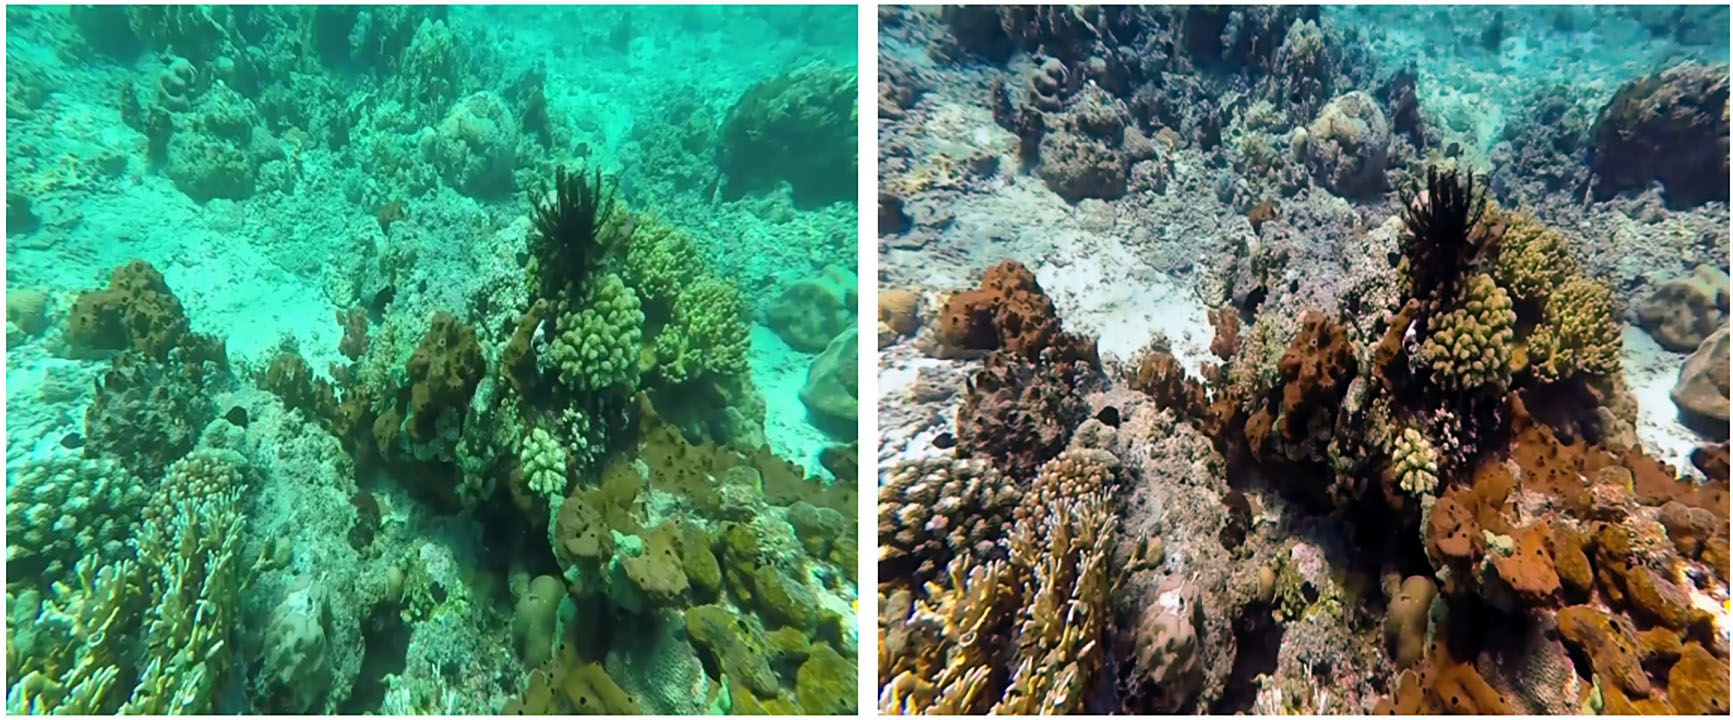
\includegraphics[width=0.8\textwidth]{FSpiralGAN_frontiers/onepicture/start_picture300.jpg}
\end{center}
$~~~~~~~~~~~~~~~~~~~~~~~~~~~~~~~~~~~~~~~~~~~~~~~~$\textbf{A} $~~~~~~~~~~~~~~~~~~~~~~~~~~~~~~~~~~~~~~~~~~~~~~~~~~~~~~~~~~~~~~~~~$\textbf{B} 
 \caption{(\textbf{A}) Raw underwater image at 960p resolution ($1280\times960$), (\textbf{B}) enhanced underwater image generated by our model at a running speed of 40 FPS.\label{fig:start picture}}
\end{figure}

\begin{figure}[htbp]
\begin{center}
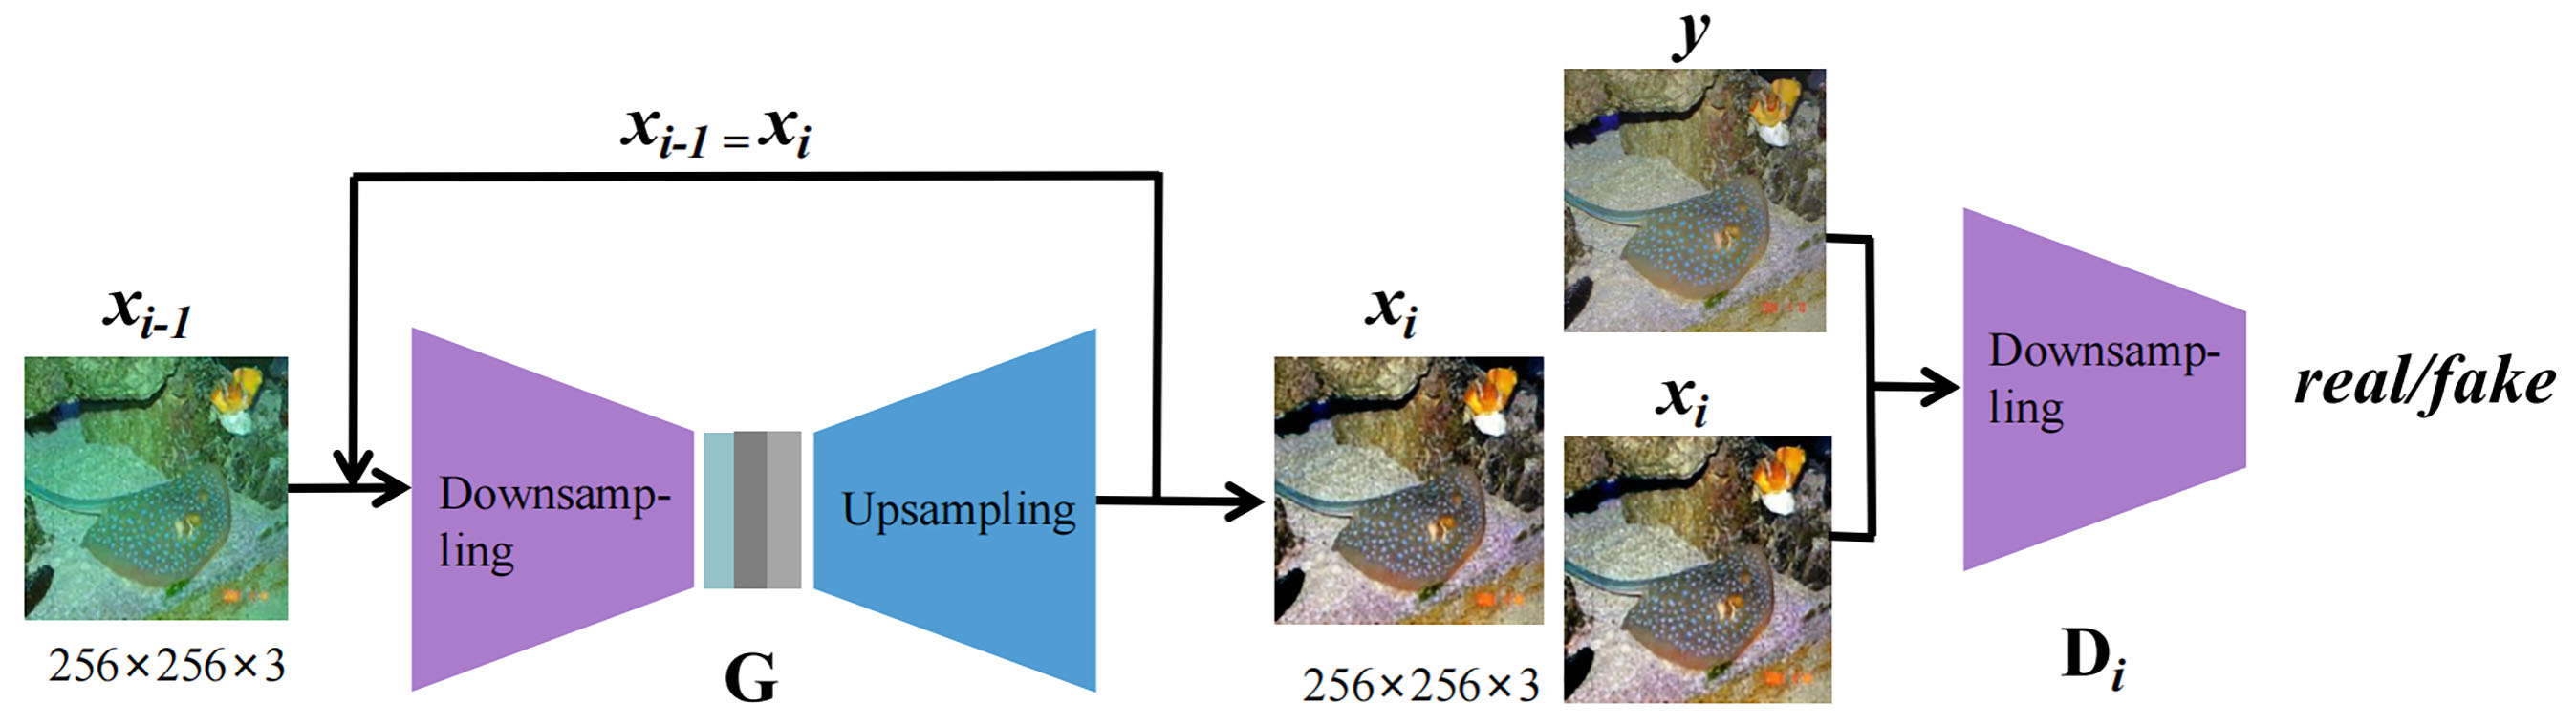
\includegraphics[width=0.8\textwidth]{FSpiralGAN_frontiers/onepicture/overrall_model300.jpg}
\end{center}
 \caption{The overall structure of our model.\label{fig:overviewofarchitecture}}
\end{figure}

\begin{figure}[htbp]
\begin{center}
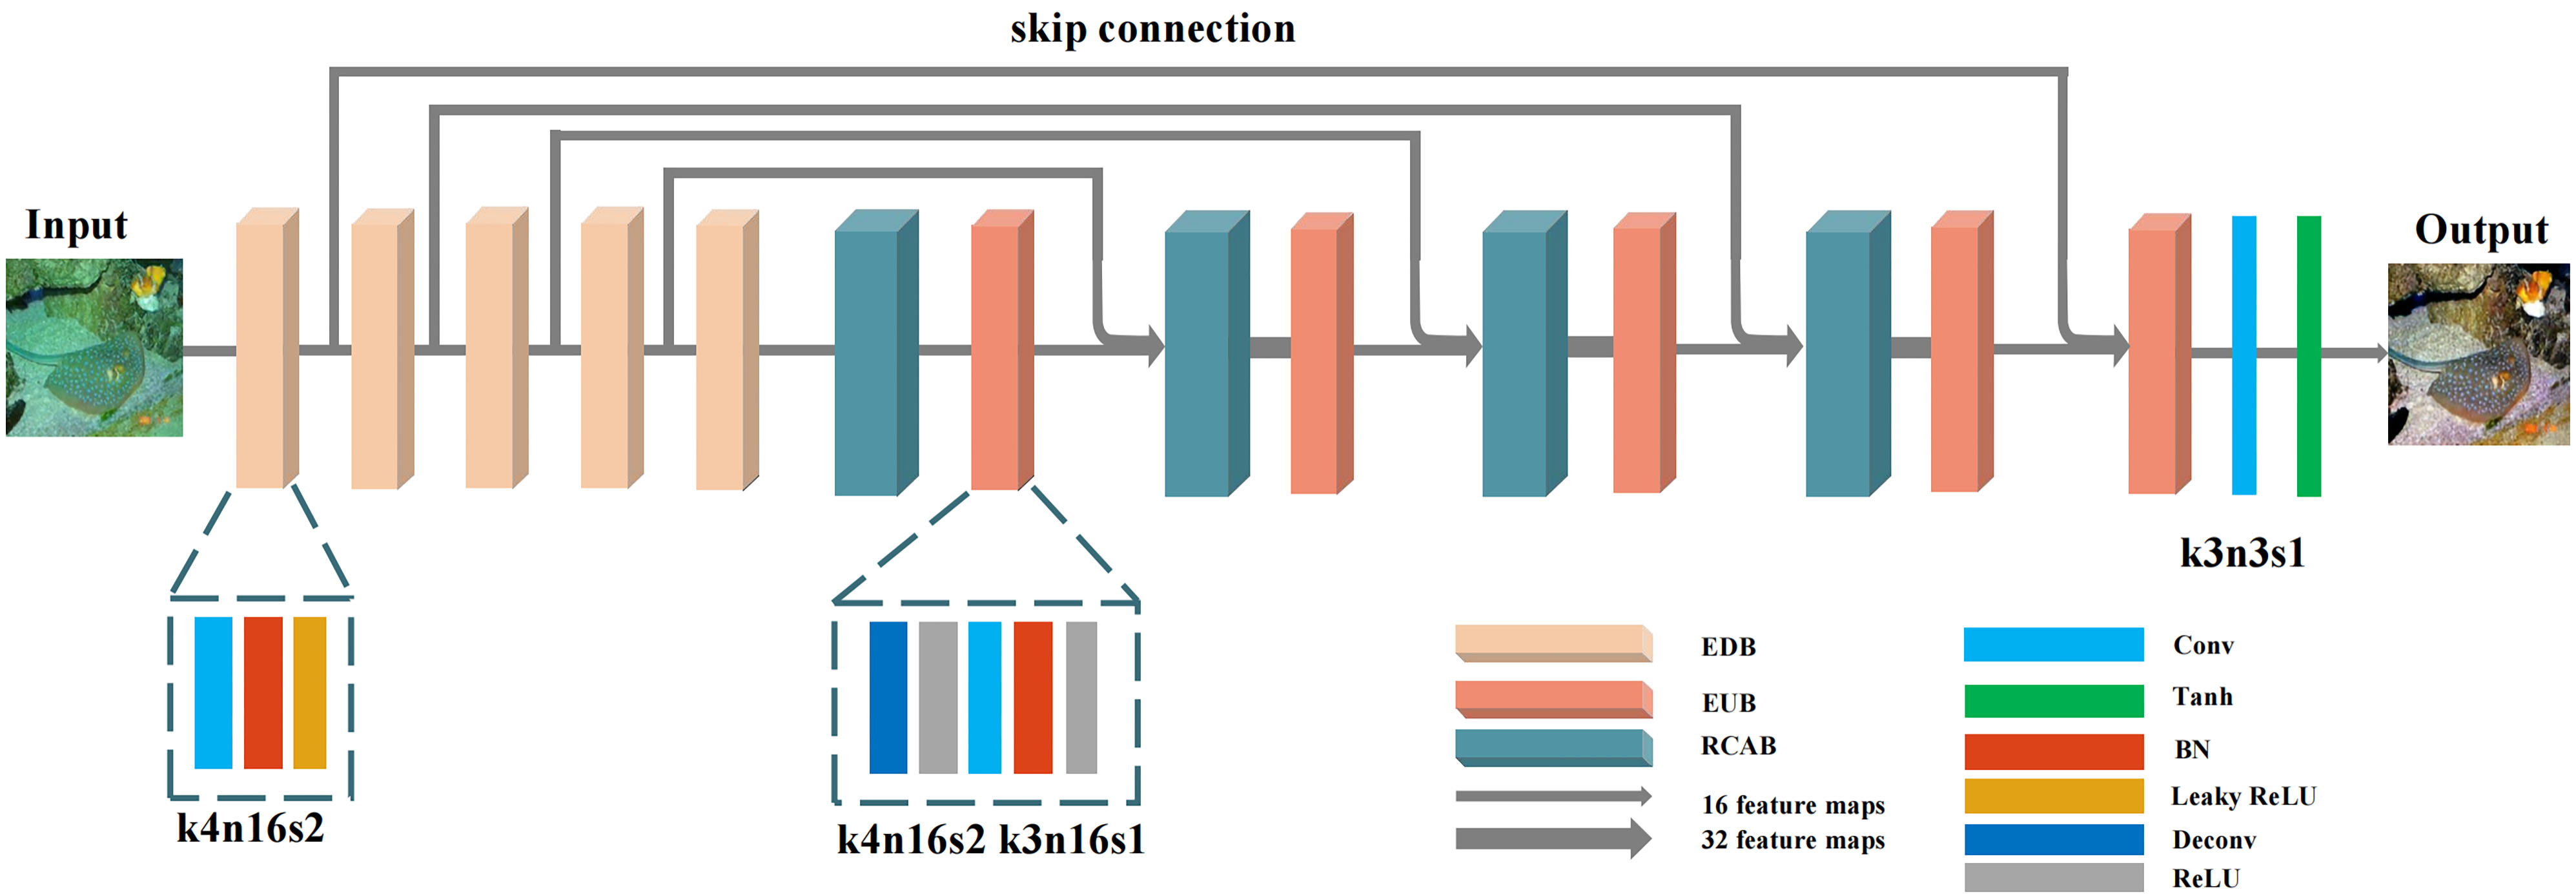
\includegraphics[width=0.8\textwidth]{FSpiralGAN_frontiers/onepicture/generator300.jpg}
\end{center}
 \caption{The architecture of the generator.\label{fig:generatorarchitecture}}
\end{figure}

\begin{figure}[htbp]
\begin{center}
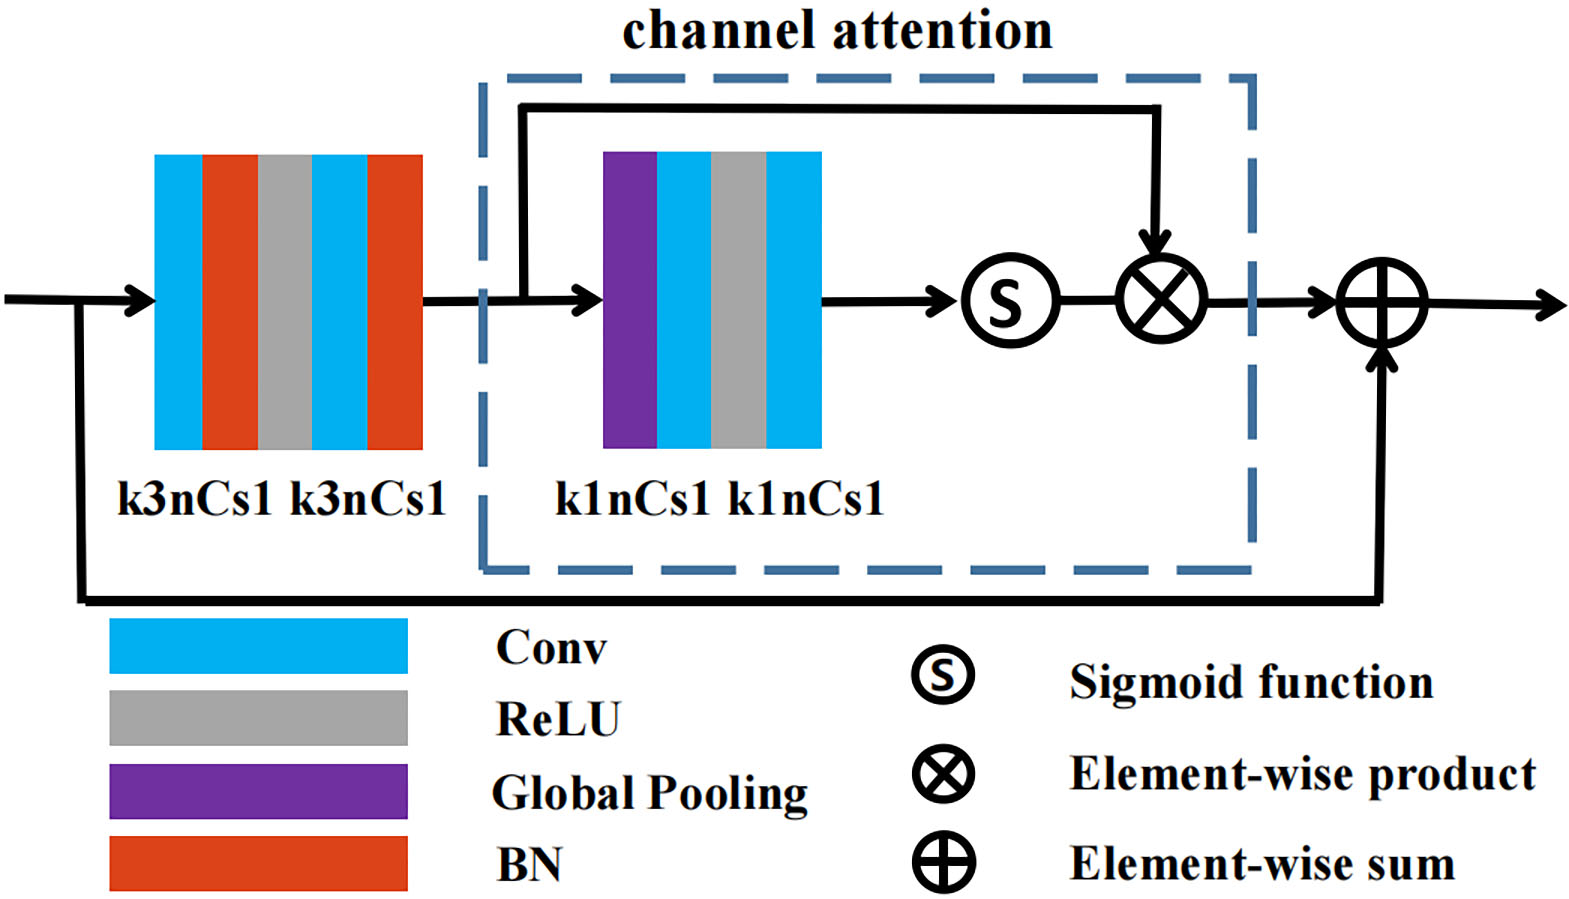
\includegraphics[width=0.4\textwidth]{FSpiralGAN_frontiers/onepicture/RCAB300.jpg}
\end{center}
 \caption{The structure of the residual channel attention block (RCAB).\label{fig:RCABarchitecture}}
\end{figure}

\begin{figure}[htbp]
\begin{center}
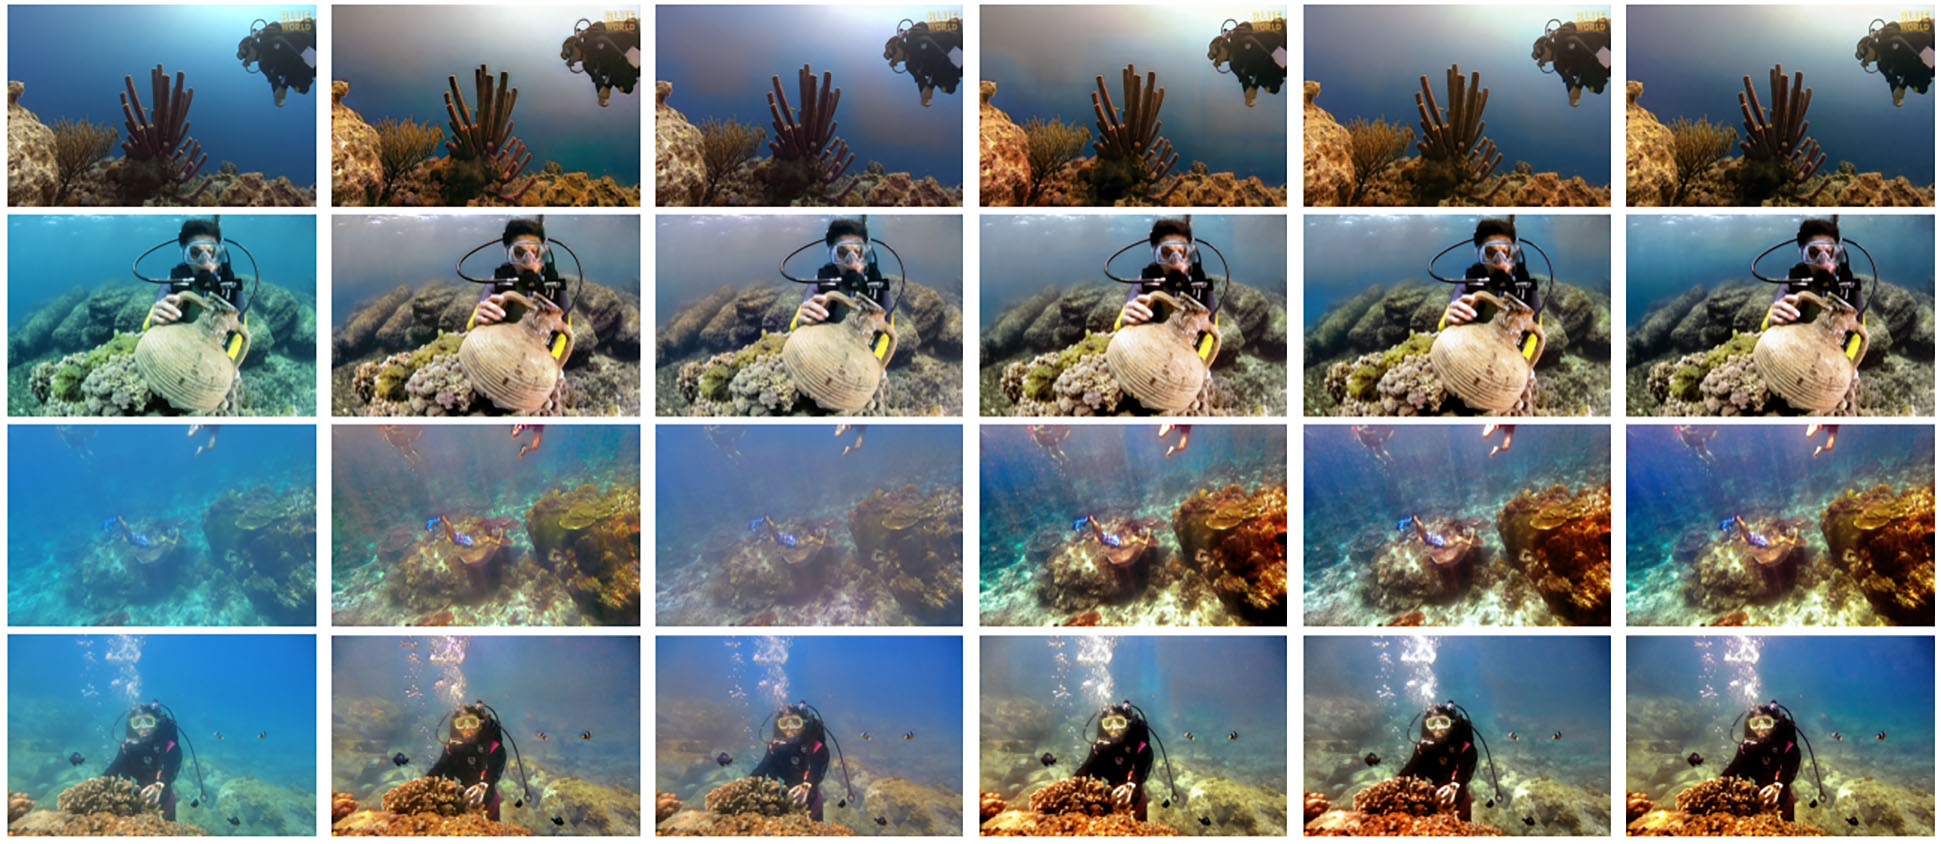
\includegraphics[width=0.9\textwidth]{FSpiralGAN_frontiers/onepicture/spatial_inconsistent300.jpg}
\end{center}
$~~~~~~~~~~~~~~~~~~~~~$\textbf{A}$~~~~~~~~~~~~~~~~~~~~~~$\textbf{B}$~~~~~~~~~~~~~~~~~~~~~~$\textbf{C}$~~~~~~~~~~~~~~~~~~~~~~$\textbf{D}$~~~~~~~~~~~~~~~~~~~~~~$\textbf{E}$~~~~~~~~~~~~~~~~~~~~~~$\textbf{F}
 \caption{The phenomenon of spatially inconsistent styles (w/o RCAB indicates that the proposed model does not use RCAB). From left to right, (\textbf{A}) shows the raw underwater images, (\textbf{B-F}) are the results of UGAN-P~\citep{8460552}, FUnIE-GAN~\citep{9001231}, Spiral-GAN~\citep{2020Underwater}, w/o RCAB and the proposed model, respectively.\label{fig:comparison-spatial_inconsistent1}}
\end{figure}

\begin{figure}[htbp]
\begin{center}
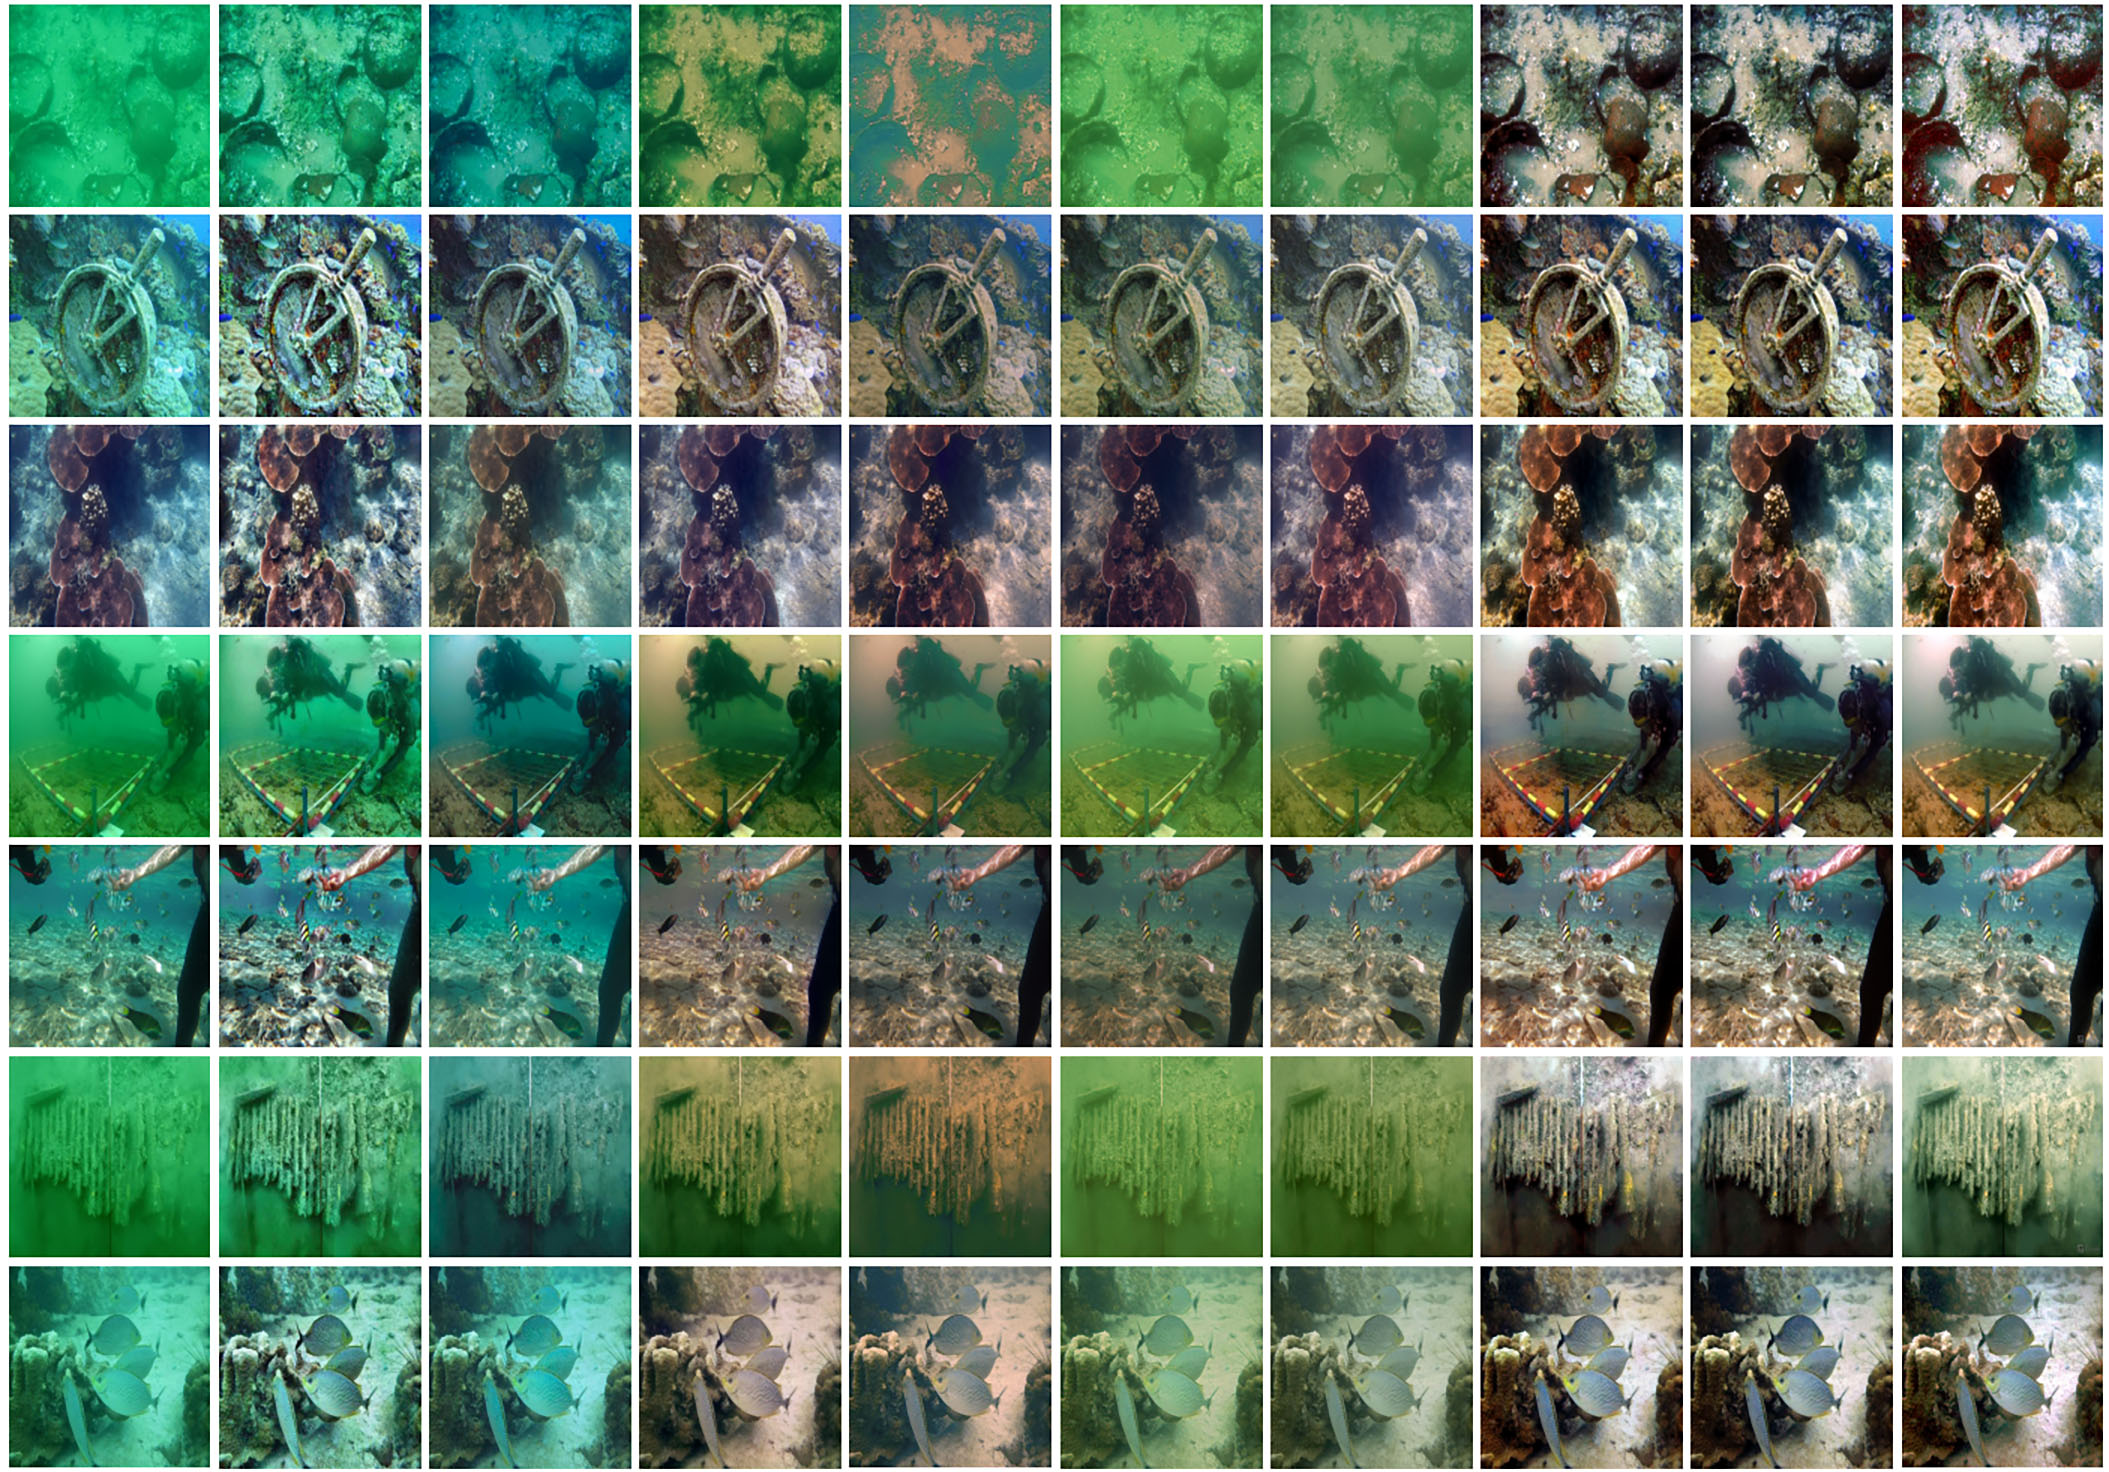
\includegraphics[width=1\textwidth]{FSpiralGAN_frontiers/onepicture/UIEB300.jpg}
\end{center}
$~~~~~~~~$\textbf{A}$~~~~~~~~~~~~~~$\textbf{B}$~~~~~~~~~~~~~~$\textbf{C}$~~~~~~~~~~~~~~$\textbf{D}$~~~~~~~~~~~~~$\textbf{E}$~~~~~~~~~~~~~~~$\textbf{F}$~~~~~~~~~~~~~~$\textbf{G}$~~~~~~~~~~~~~$\textbf{H}$~~~~~~~~~~~~~~$\textbf{I}$~~~~~~~~~~~~~~~~$\textbf{J}
 \caption{Visual comparisons on the UIEB dataset. From left to right, (\textbf{A}) shows the raw underwater images, (\textbf{B-I}) are the results of CLAHE~\citep{109340}, OMGD~\citep{ren2021online}, FUnIE-GAN~\citep{9001231}, WaterNet~\citep{8917818}, UWCNN~\citep{2019Underwater1}, Shallow-UWnet~\citep{naik2021shallow}, Spiral-GAN~\citep{2020Underwater} and the proposed model, respectively, and (\textbf{J}) shows the reference images.\label{fig:comparison-UIEBD}}
\end{figure}
\begin{table*}[htbp]\normalsize
\centering
\setlength\tabcolsep{3pt}
\caption{{Quantitative evaluation on the UIEB dataset.}}
\begin{tabular}{c|cccccccc}
\hline  
Method&CLAHE&OMGD&FUnIE-GAN&WaterNet&UWCNN&Shallow-UWnet&Spiral-GAN&Ours\\
\hline 
SSIM&\textbf{0.8459}&0.8002&0.7481&0.6902&0.6977&0.8198&0.8435&0.8450\\
\hline 
PSNR&18.58&18.51&16.91&15.06&14.61&18.18&19.02&\textbf{19.16}\\
\hline
PCQI&\textbf{0.9783}&0.6366&0.7263&0.6027&0.6017&0.6693&0.8440&0.8226\\
\hline
\end{tabular}
\label{tbl:comparison-UIEBD}
\end{table*}

\begin{figure}[htbp]
\begin{center}
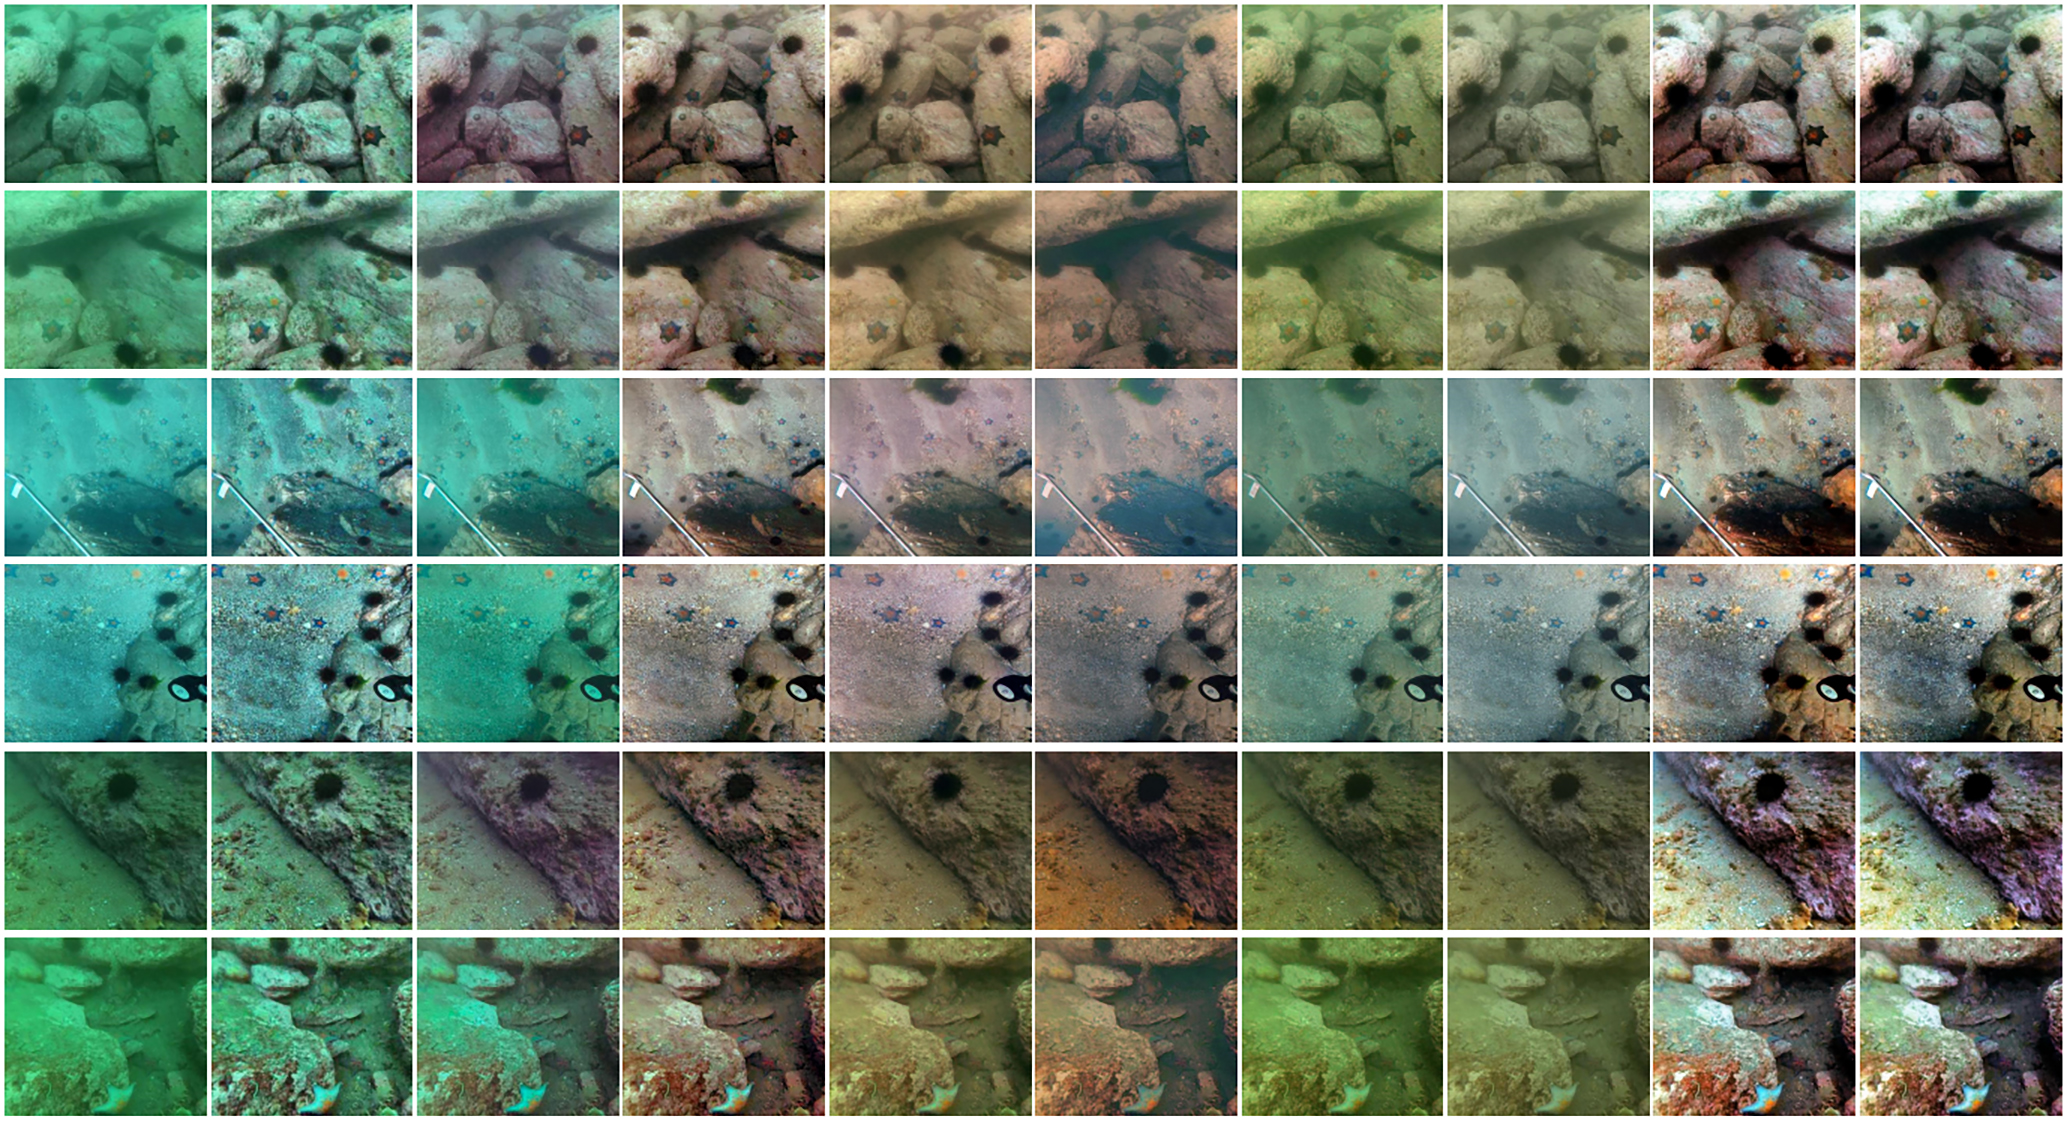
\includegraphics[width=1\textwidth]{FSpiralGAN_frontiers/onepicture/UCCS300.jpg}
\end{center}
$~~~~~~~~$\textbf{A}$~~~~~~~~~~~~~$\textbf{B}$~~~~~~~~~~~~~~$\textbf{C}$~~~~~~~~~~~~~~$\textbf{D}$~~~~~~~~~~~~~~$\textbf{E}$~~~~~~~~~~~~~~$\textbf{F}$~~~~~~~~~~~~~~~$\textbf{G}$~~~~~~~~~~~~~$\textbf{H}$~~~~~~~~~~~~~~~$\textbf{I}$~~~~~~~~~~~~~~$\textbf{J}
 \caption{{Visual comparisons on the UCCS subset of the RUIE dataset. From left to right, (\textbf{A}) shows the raw underwater images, (\textbf{B-J}) are the results of CLAHE~\citep{109340}, OMGD~\citep{ren2021online}, UGAN-P~\citep{8460552}, FUnIE-GAN~\citep{9001231}, WaterNet~\citep{8917818}, UWCNN~\citep{2019Underwater1}, Shallow-UWnet~\citep{naik2021shallow}, Spiral-GAN~\citep{2020Underwater} and the proposed model, respectively.}\label{fig:comparison-3part}}
\end{figure}

\begin{table*}[htbp]\small
\centering
\setlength\tabcolsep{3pt}
\caption{{Quantitative evaluation on the UCCS subset of the RUIE dataset.}}
\begin{tabular}{c|ccccccccc}
\hline  
Method&CLAHE&OMGD&UGAN-P&FUnIE-GAN&WaterNet&UWCNN&Shallow-UWnet&Spiral-GAN&Ours\\
\hline 
UISM&6.521&\textbf{6.749}&6.611&6.739&6.623&6.606&6.703&6.544&6.473\\
\hline 
UICM&1.791&2.917&1.905&1.131&2.955&0.864&0.742&2.892&\textbf{3.336}\\
\hline 
UIConM&0.743&0.681&0.699&0.603&0.626&0.580&0.512&0.724&\textbf{0.807}\\
\hline 
UIQM&4.631&4.511&4.498&4.179&4.277&4.050&3.830&4.602&\textbf{4.892}\\
\hline 
UCIQE&0.493&0.5181&0.547&0.4957&0.4999&0.4579&0.4397&0.6137&\textbf{0.6148}\\
\hline
CCF&20.14&14.01&18.85&14.51&12.68&12.24&11.83&\textbf{27.64}&26.43\\
\hline
\end{tabular}
\label{tbl:comparison-3part}
\end{table*}

\begin{figure}[htbp]
\begin{center}
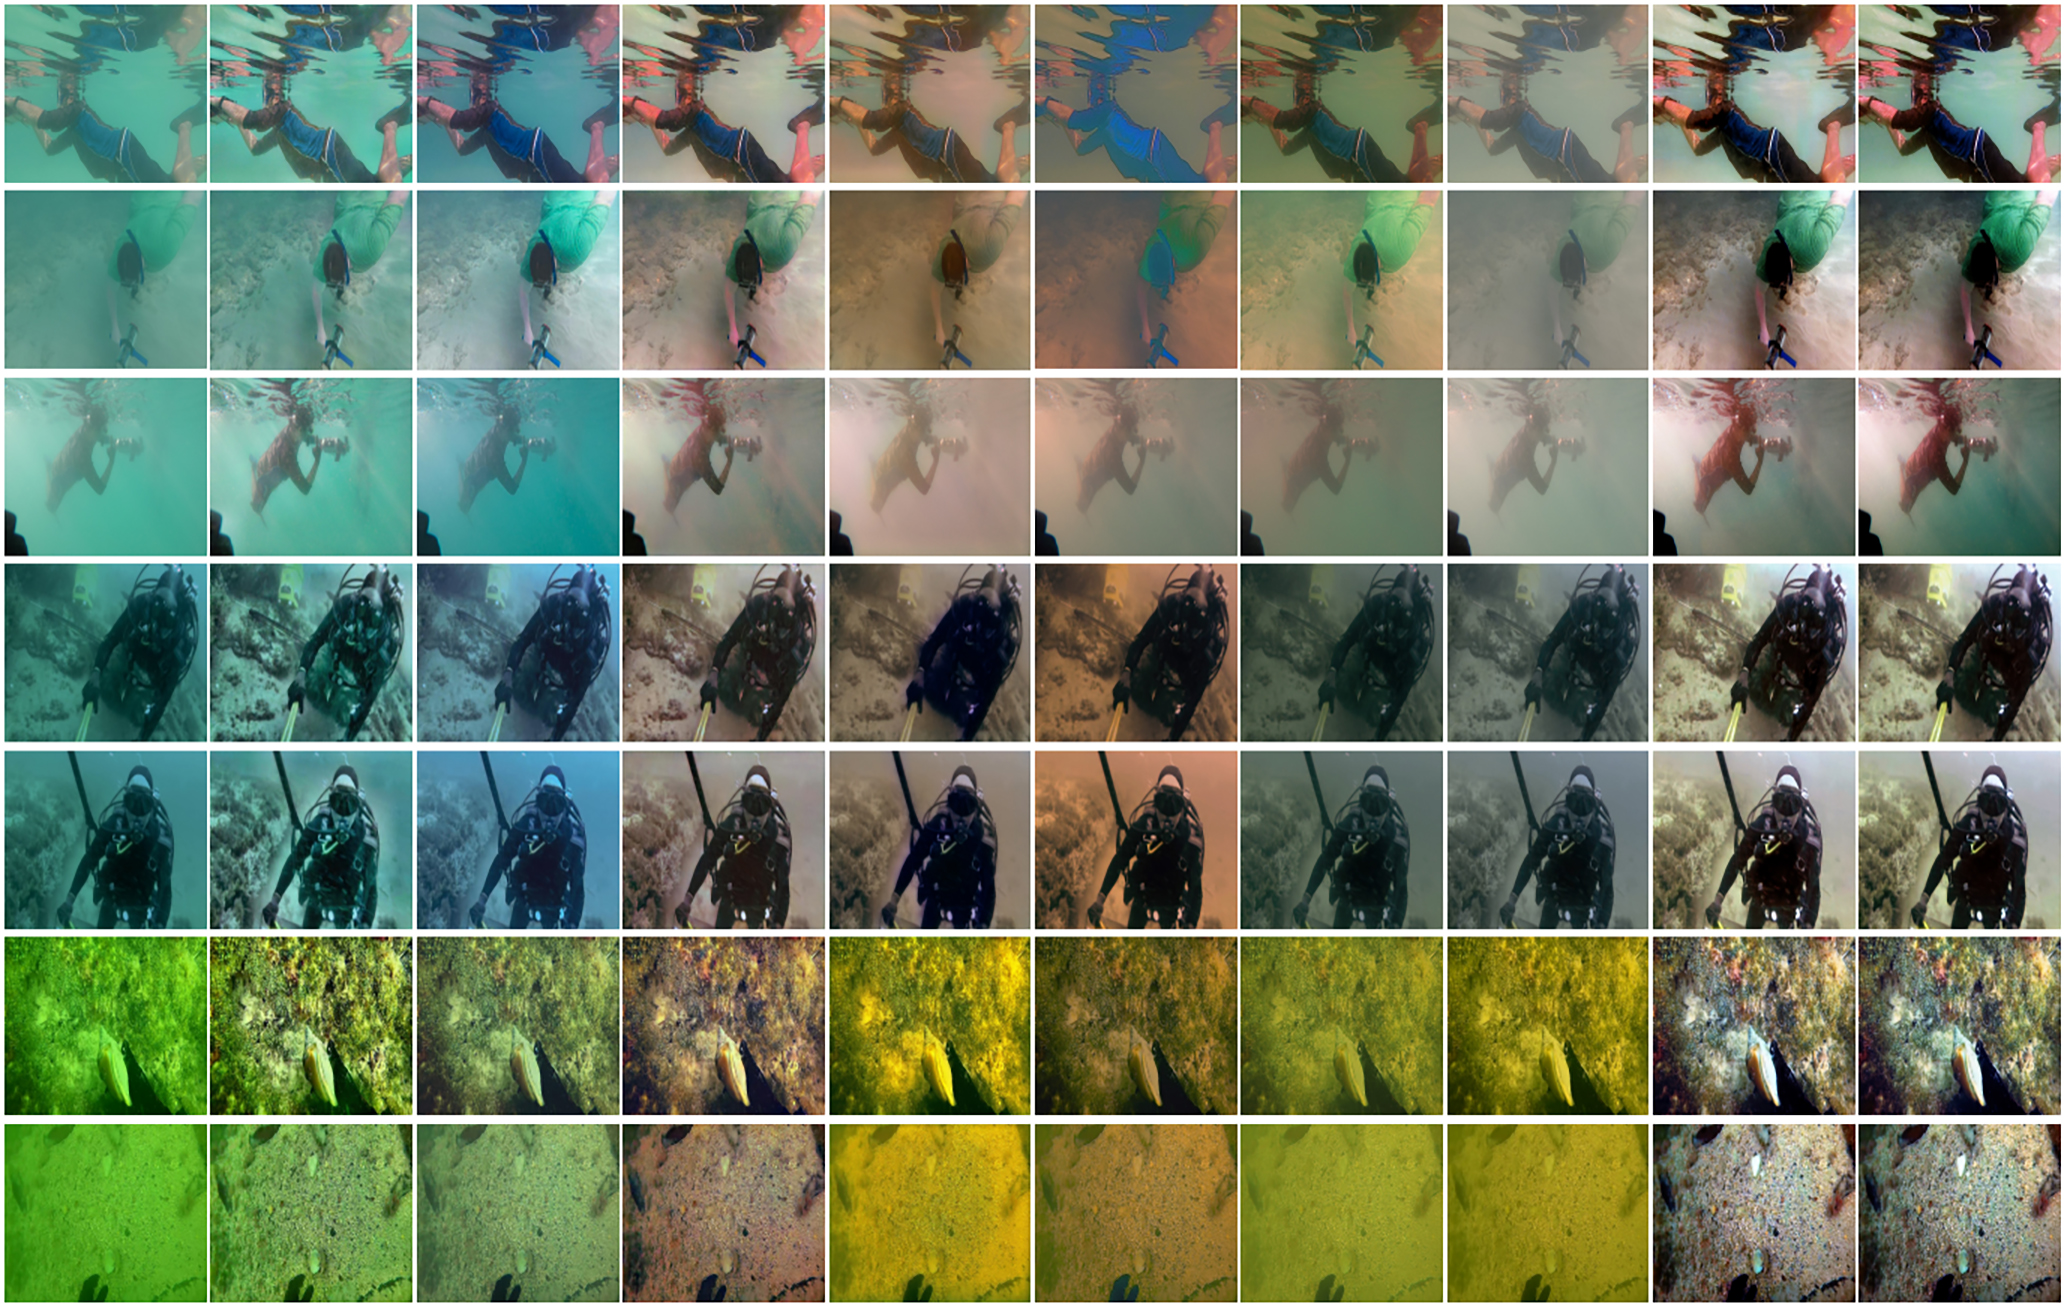
\includegraphics[width=1\textwidth]{FSpiralGAN_frontiers/onepicture/EUVP300.jpg}
\end{center}
$~~~~~~~~$\textbf{A}$~~~~~~~~~~~~~$\textbf{B}$~~~~~~~~~~~~~~$\textbf{C}$~~~~~~~~~~~~~~~$\textbf{D}$~~~~~~~~~~~~~~$\textbf{E}$~~~~~~~~~~~~~~$\textbf{F}$~~~~~~~~~~~~~~$\textbf{G}$~~~~~~~~~~~~~~$\textbf{H}$~~~~~~~~~~~~~~$\textbf{I}$~~~~~~~~~~~~~~$\textbf{J}
 \caption{{Visual comparisons on the EUVP dataset. From left to right, (\textbf{A}) shows the raw underwater images, (\textbf{B-J}) are the results of CLAHE~\citep{109340}, OMGD~\citep{ren2021online}, UGAN-P~\citep{8460552}, FUnIE-GAN~\citep{9001231}, WaterNet~\citep{8917818}, UWCNN~\citep{2019Underwater1}, Shallow-UWnet~\citep{naik2021shallow}, Spiral-GAN~\citep{2020Underwater} and the proposed model, respectively.}\label{fig:comparison-fgan}}
\end{figure}

\begin{table*}[htbp]\small
\centering
\setlength\tabcolsep{3pt}
\caption{{Quantitative evaluation on the EUVP dataset.}}
\begin{tabular}{c|ccccccccc}
\hline  
Method&CLAHE&OMGD&UGAN-P&FUnIE-GAN&WaterNet&UWCNN&Shallow-UWnet&Spiral-GAN&Ours\\
\hline 
UISM&7.191&6.968&6.827&7.128&6.984&7.139&\textbf{7.298}&6.873&6.864\\
\hline 
UICM&1.405&2.354&2.318&0.677&4.335&1.219&0.889&3.438&\textbf{4.370}\\
\hline 
UIConM&0.542&0.560&0.608&0.439&0.531&0.473&0.354&0.767&\textbf{0.852}\\
\hline 
UIQM&4.101&4.125&4.255&3.693&4.083&3.834&3.446&4.868&\textbf{5.146}\\
\hline 
UCIQE&0.440&0.4857&0.530&0.4313&0.4812&0.4356&0.3975&0.6166&\textbf{0.6213}\\
\hline
CCF&13.68&11.46&14.33&10.06&9.75&8.90&9.30&\textbf{22.87}&21.08\\
\hline
\end{tabular}
\label{tbl:comparison-fgan}
\end{table*}


\begin{figure}[htbp]
\begin{center}
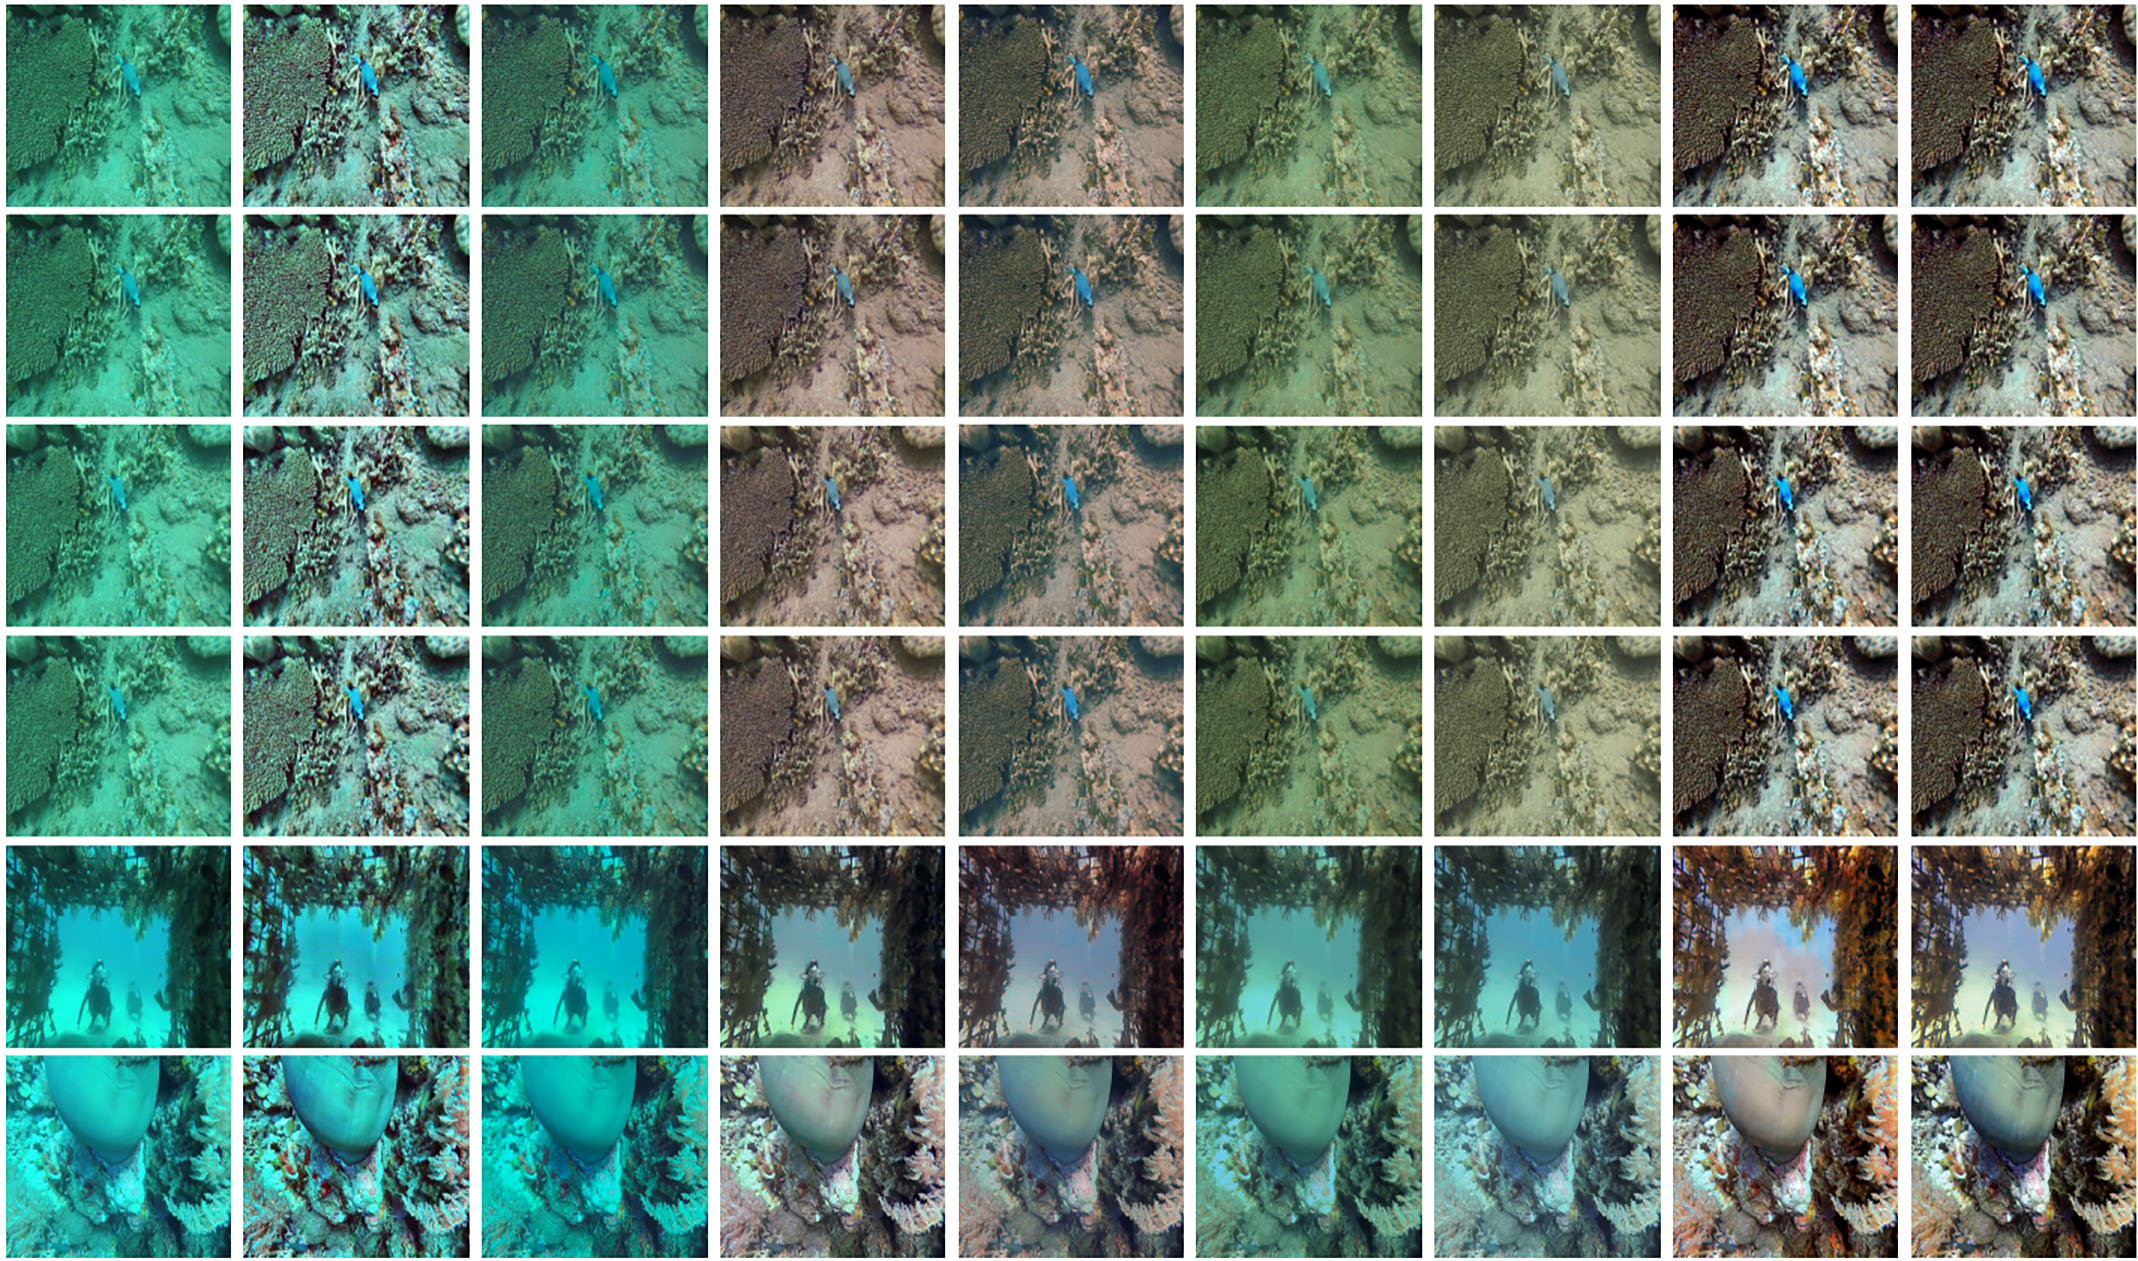
\includegraphics[width=1\textwidth]{FSpiralGAN_frontiers/onepicture/underwater_video300.jpg}
\end{center}
$~~~~~~~~$\textbf{A}$~~~~~~~~~~~~~~~~$\textbf{B}$~~~~~~~~~~~~~~~~$\textbf{C}$~~~~~~~~~~~~~~~~$\textbf{D}$~~~~~~~~~~~~~~~~$\textbf{E}$~~~~~~~~~~~~~~~~$\textbf{F}$~~~~~~~~~~~~~~~~$\textbf{G}$~~~~~~~~~~~~~~~$\textbf{H}$~~~~~~~~~~~~~~~~~$\textbf{I}
 \caption{Visual comparisons of the 1280$\times$960 frames in the underwater video. From left to right, (\textbf{A}) shows the raw underwater images, (\textbf{B-I}) are the results of CLAHE~\citep{109340}, OMGD~\citep{ren2021online}, FUnIE-GAN~\citep{9001231}, WaterNet~\citep{8917818}, UWCNN~\citep{2019Underwater1}, Shallow-UWnet~\citep{naik2021shallow}, Spiral-GAN~\citep{2020Underwater} and the proposed model, respectively.\label{fig:comparison-underwater video}}
\end{figure}

\begin{table*}[htbp]\normalsize
\centering
\setlength\tabcolsep{2.7pt}
\caption{Frames per second (FPS) of different methods on the underwater video.}
\begin{tabular}{c|ccccccccc}
\hline  
Method&CLAHE&OMGD&FUnIE-GAN&WaterNet&UWCNN&Shallow-UWnet&Spiral-GAN&Ours\\
\hline 
1280$\times$960&137.7&20.4&13.1&1.5&10.6&7.1&22.4&\textbf{40.0}\\
\hline
256$\times$256&820.7&185.0&36.1&15.2&\textbf{267.7}&68.4&222.8&246.3\\
\hline 
\end{tabular}
\label{tbl:comparison-underwatervideo1}
\end{table*}

\begin{table*}[htbp]\normalsize
\centering
\setlength\tabcolsep{2pt}
\caption{Parameters and FLOPs of different methods on the 1280$\times$960 underwater video.}
\begin{tabular}{c|ccccccccc}
\hline  
Method&CLAHE&OMGD&FUnIE-GAN&WaterNet&UWCNN&Shallow-UWnet&Spiral-GAN&Ours\\
\hline 
Parameters&-&137347&4215843&1090668&\textbf{39972}&219456&4993539&133987\\
\hline 
FLOPs(G)&-&53&233&2679&98&406&138&\textbf{20}\\
% \hline
% FPS(img/s)&137.7&13.1&1.5&10.6&7.1&22.4&\textbf{40.0}\\
\hline 
\end{tabular}
\label{tbl:comparison-underwatervideo}
\end{table*}

\begin{figure}[htbp]
\begin{center}
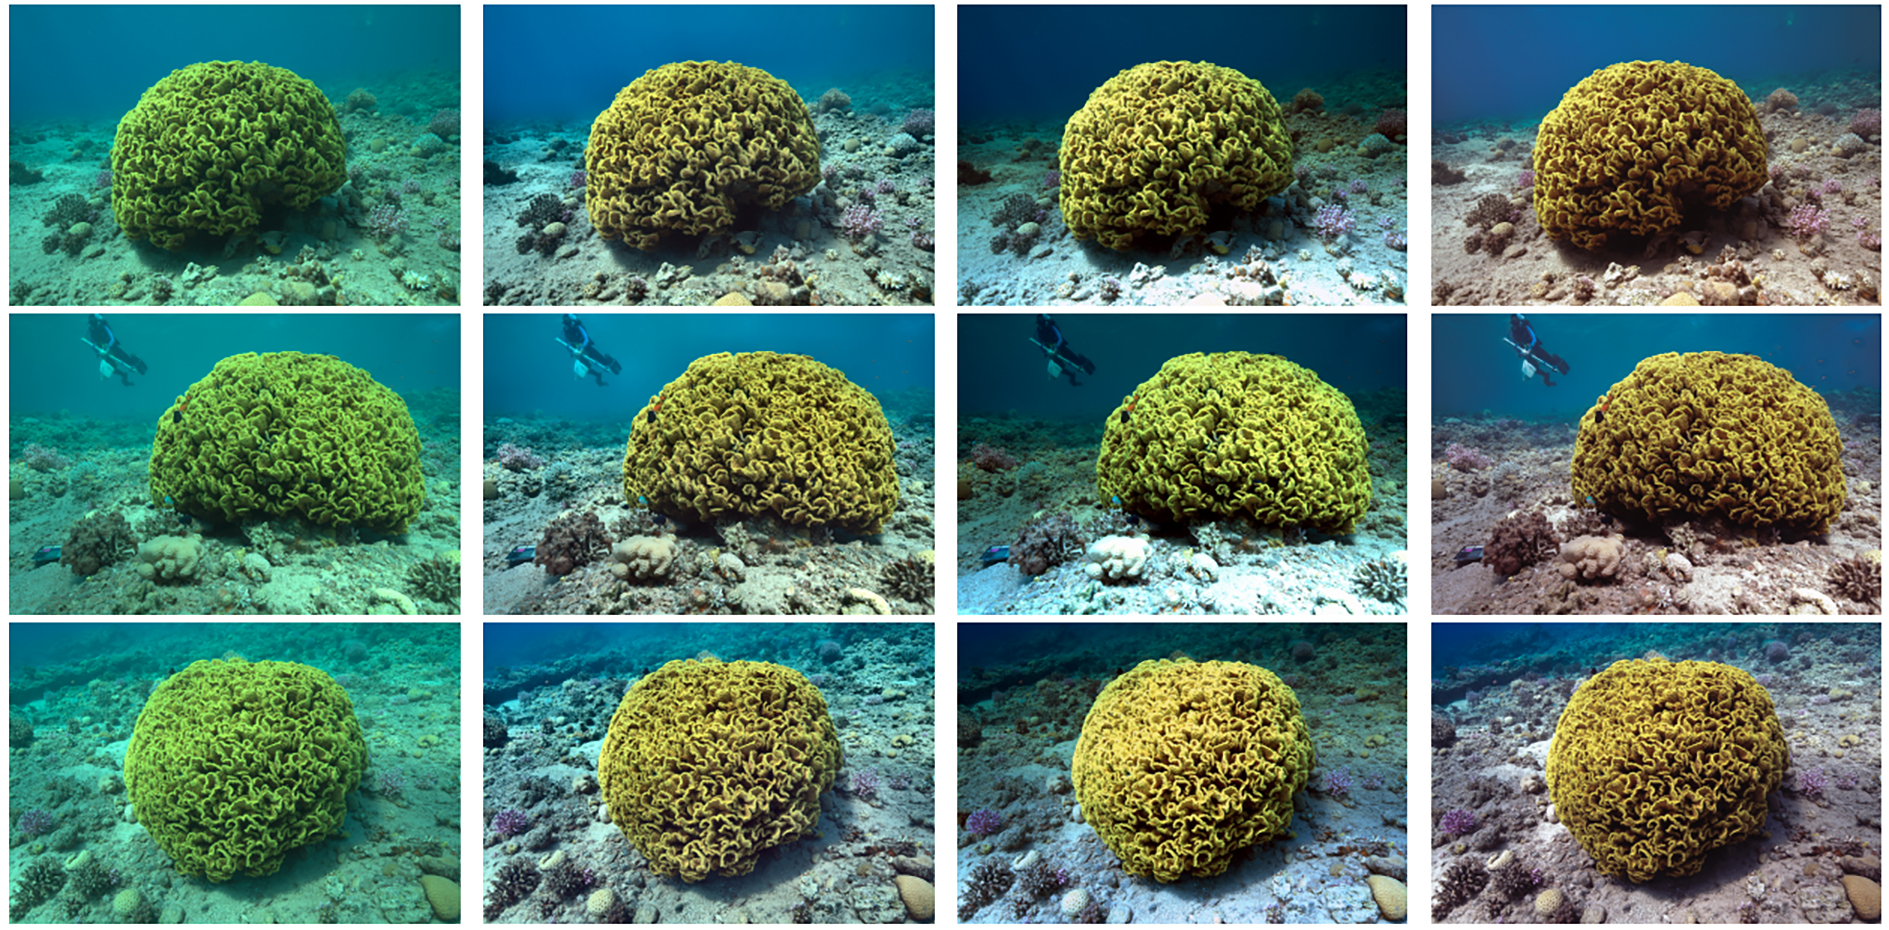
\includegraphics[width=1\textwidth]{FSpiralGAN_frontiers/onepicture/D3300.jpg}
\end{center}
$~~~~~~~~~~~~~~~~~~~~$\textbf{A}$~~~~~~~~~~~~~~~~~~~~~~~~~~~~~~~~~~~~~~~~$\textbf{B}$~~~~~~~~~~~~~~~~~~~~~~~~~~~~~~~~~~~~~~~~$\textbf{C}$~~~~~~~~~~~~~~~~~~~~~~~~~~~~~~~~~~~~~$\textbf{D}
 \caption{{Visual comparisons on the 7968$\times$5312 images in the D3 dataset. From left to right, (\textbf{A}) shows the raw underwater images, (\textbf{B-I}) are the results of Fusion~\citep{2012Enhancing}, Sea-thru~\citep{akkaynak2019sea} and the proposed model, respectively.} \label{fig:D3}}
\end{figure}

\begin{table}[htbp]\normalsize
\centering
\setlength\tabcolsep{15pt}
\caption{{Quantitative evaluation on 7968$\times$5312 images.}}
\begin{tabular}{c|ccc}
\hline  
Methods&FPS&UCIQE&UIQM\\
\hline 
Fusion&0.0061&0.653&4.630\\ 
\hline
Sea-thru&0.0003&\textbf{0.674}&\textbf{4.783}\\
\hline
Ours&\textbf{0.9118}&0.667&4.690\\
\hline 
\end{tabular}
\label{tbl:D3}
\end{table}

\begin{figure}[htbp]
\begin{center}
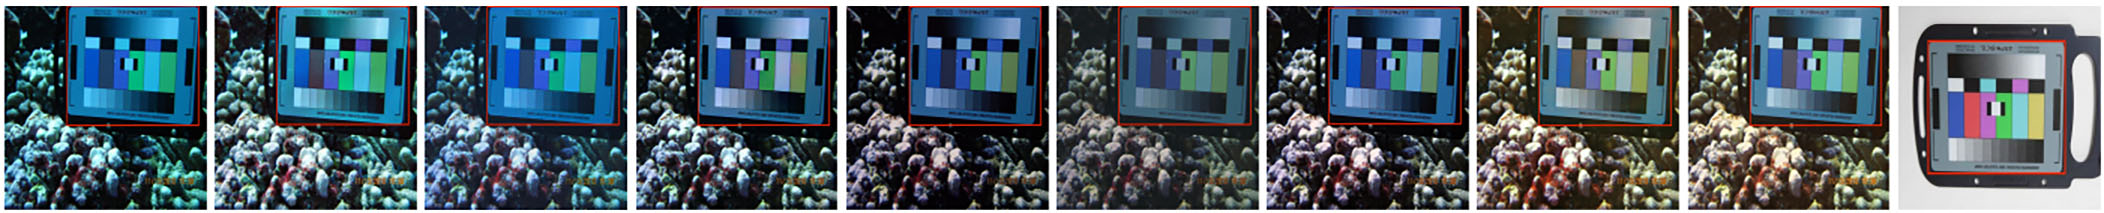
\includegraphics[width=1\textwidth]{FSpiralGAN_frontiers/onepicture/color_card300.jpg}
\end{center}
$~~~~~~~~$\textbf{A}$~~~~~~~~~~~~~~$\textbf{B}$~~~~~~~~~~~~~~$\textbf{C}$~~~~~~~~~~~~~~$\textbf{D}$~~~~~~~~~~~~~$\textbf{E}$~~~~~~~~~~~~~~~$\textbf{F}$~~~~~~~~~~~~~~$\textbf{G}$~~~~~~~~~~~~~$\textbf{H}$~~~~~~~~~~~~~~$\textbf{I}$~~~~~~~~~~~~~~~~$\textbf{J}
 \caption{The visual results of the color accuracy test. From left to right, (\textbf{A}) shows the raw underwater images, (\textbf{B-I}) are the results of CLAHE~\citep{109340}, OMGD~\citep{ren2021online}, FUnIE-GAN~\citep{9001231}, WaterNet~\citep{8917818}, UWCNN~\citep{2019Underwater1}, Shallow-UWnet~\citep{naik2021shallow}, Spiral-GAN~\citep{2020Underwater} and the proposed model, respectively, and (\textbf{J}) shows the reference images.\label{fig:colorcard}}
\end{figure}

\begin{table*}[htbp]\normalsize
\setlength\tabcolsep{4pt}
\centering
\caption{The result of mutual information.}
\begin{tabular}{c|cccccccc}
\hline  
Method&CLAHE&OMGD&FUnIE-GAN&WaterNet&UWCNN&SUWnet&Spiral-GAN&Ours\\
\hline 
score&0.547&0.6416&0.623&0.691&0.701&0.695&0.644&\textbf{0.722}\\ 
\hline
\end{tabular}
\label{tbl:colorcard}
\end{table*}

\begin{figure}[htbp]
\begin{center}
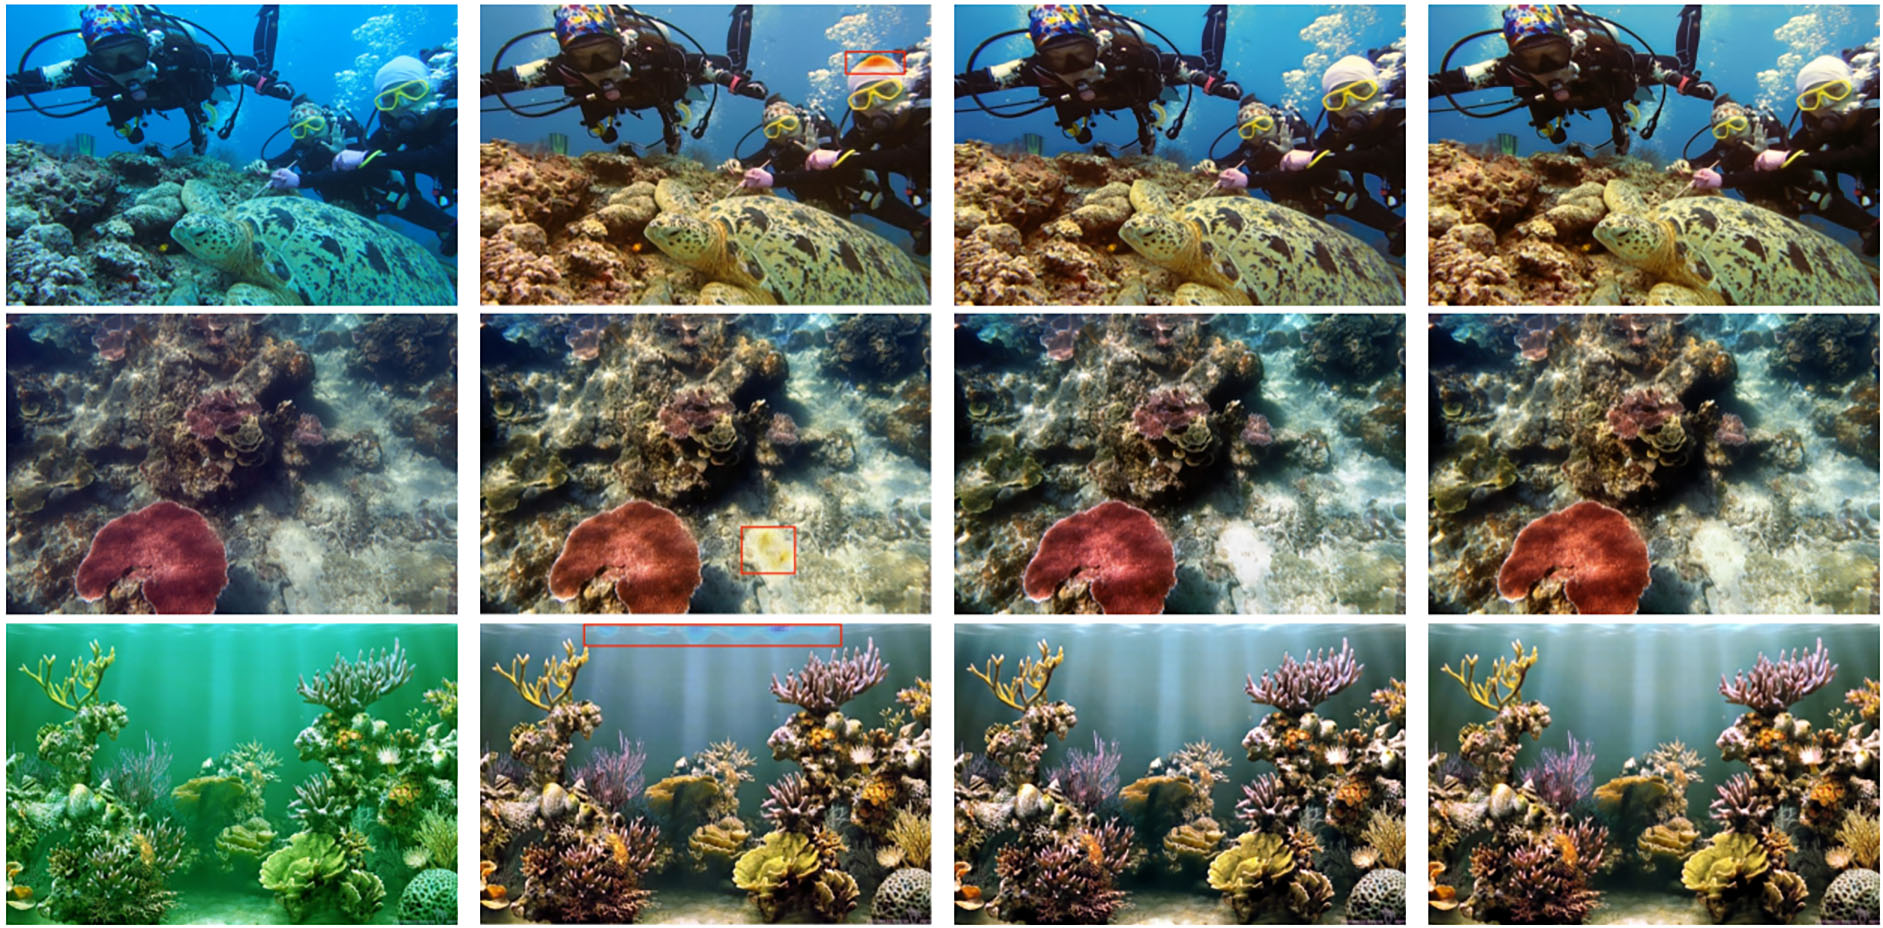
\includegraphics[width=1\textwidth]{FSpiralGAN_frontiers/onepicture/abalation_channel300.jpg}
\end{center}
$~~~~~~~~~~~~~~~~~~~~$\textbf{A}$~~~~~~~~~~~~~~~~~~~~~~~~~~~~~~~~~~~~~~~~$\textbf{B}$~~~~~~~~~~~~~~~~~~~~~~~~~~~~~~~~~~~~~~~~$\textbf{C}$~~~~~~~~~~~~~~~~~~~~~~~~~~~~~~~~~~~~~$\textbf{D}
 \caption{Visual comparisons with different network widths $C$ in EDB and EUB on the UIEB dataset. From left to right, (\textbf{A}) shows the raw underwater images, and (\textbf{B-D}) are the results of $C=8$, $C=16$ and $C=32$, respectively. \label{fig:ablationchannel-UIEBD}}
\end{figure}

\begin{table}[htbp]\normalsize
\centering
\setlength\tabcolsep{13pt}
\caption{{PCQI, SSIM, PSNR, and FPS comparison on the UIEB dataset using different network widths.}}
\begin{tabular}{c|cccc}
\hline  
Method&PCQI&SSIM&PSNR&FPS\\
\hline 
C=8&0.7909&0.839&19.28&55\\ 
\hline
C=16&0.8226&0.845&19.164&40\\
\hline
C=32&0.8402&0.854&19.462&25\\
\hline 
\end{tabular}
\label{tbl:ablationchannel-UIEBD}
\end{table}

\begin{figure}[htbp]
\begin{center}
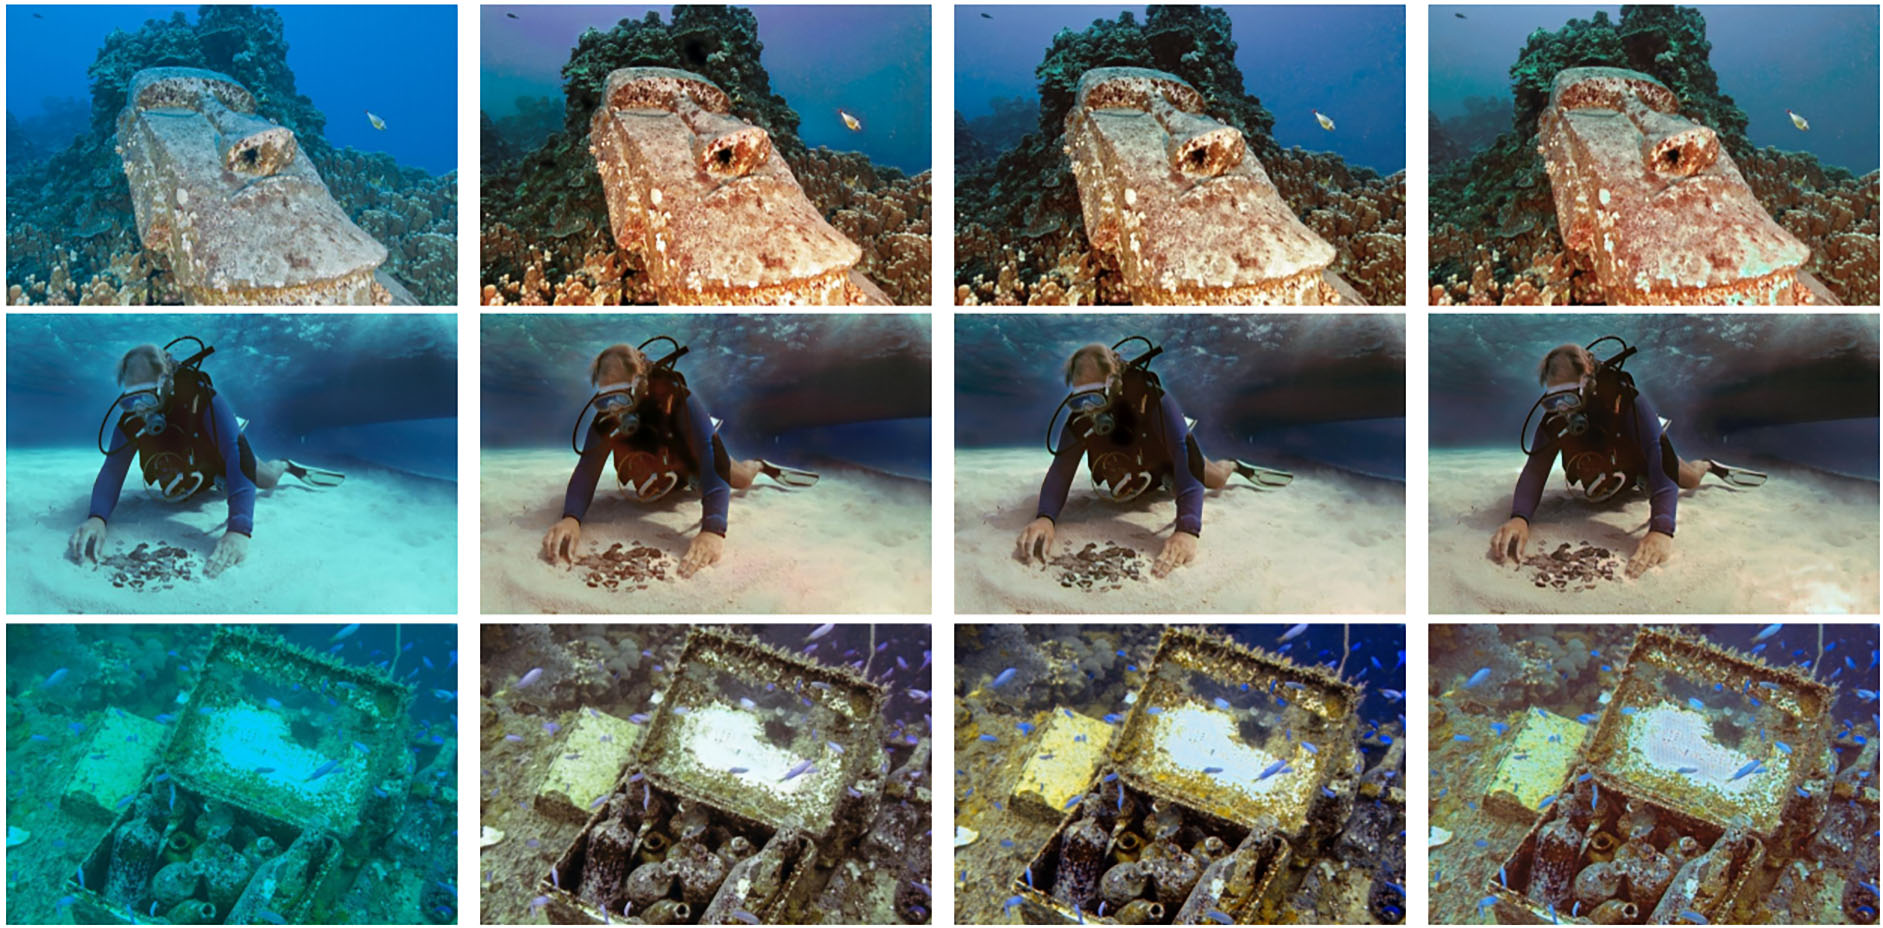
\includegraphics[width=1\textwidth]{FSpiralGAN_frontiers/onepicture/abalation_RCAB300.jpg}
\end{center}
$~~~~~~~~~~~~~~~~~~~~$\textbf{A}$~~~~~~~~~~~~~~~~~~~~~~~~~~~~~~~~~~~~~~~~$\textbf{B}$~~~~~~~~~~~~~~~~~~~~~~~~~~~~~~~~~~~~~~~~$\textbf{C}$~~~~~~~~~~~~~~~~~~~~~~~~~~~~~~~~~~~~~$\textbf{D}
 \caption{Visual comparisons with different RCAB numbers $N$ in the generator on the UIEB dataset. From left to right, (\textbf{A}) shows the raw underwater images, and (\textbf{B-D}) are the results of $N=3$, $N=4$(Ours) and $N=5$, respectively. \label{fig:ablationRCAB-UIEBD}}
\end{figure}

\begin{table}[htbp]\normalsize
\centering
\setlength\tabcolsep{13pt}
\caption{{PCQI, SSIM, PSNR, and FPS comparison on the UIEB dataset using different RCAB numbers.}}
\begin{tabular}{c|cccc}
\hline  
Method&PCQI&SSIM&PSNR&FPS\\
\hline 
N=3&0.8107&0.844&18.961&\textbf{41}\\ 
\hline
N=4(Ours)&\textbf{0.8226}&\textbf{0.845}&\textbf{19.164}&40\\
\hline
N=5&0.7942&0.843&18.972&32\\
\hline 
\end{tabular}
\label{tbl:ablationRCAB-UIEBD}
\end{table}

\begin{figure}[htbp]
\begin{center}
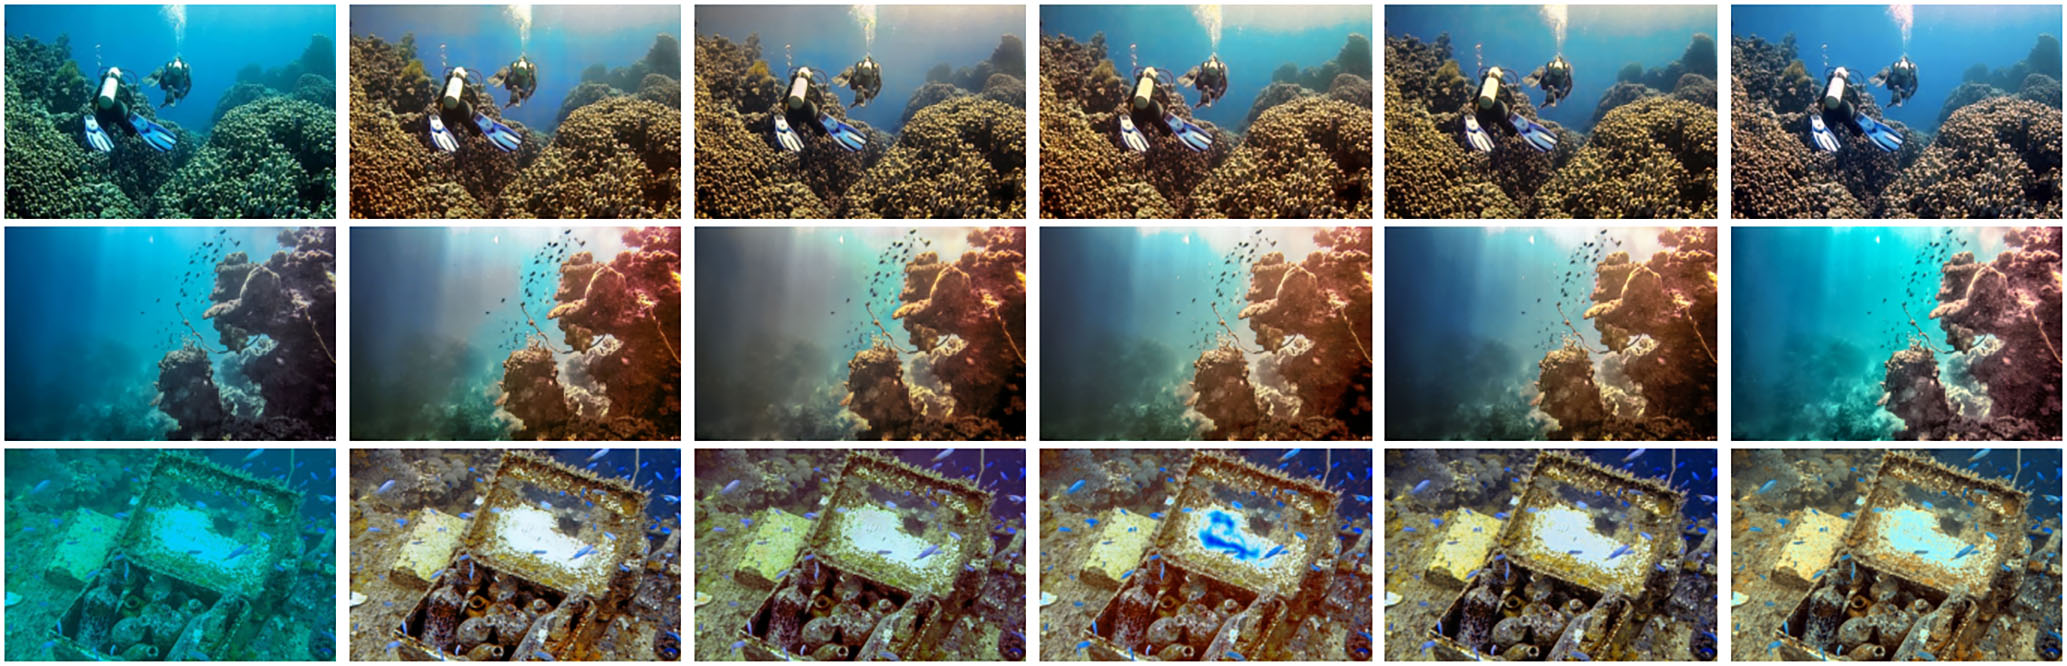
\includegraphics[width=1\textwidth]{FSpiralGAN_frontiers/onepicture/abalation_BN300.jpg}
\end{center}
$~~~~~~~~~~~~~$\textbf{A}$~~~~~~~~~~~~~~~~~~~~~~~~~$\textbf{B}$~~~~~~~~~~~~~~~~~~~~~~~~~$\textbf{C}$~~~~~~~~~~~~~~~~~~~~~~~~~~$\textbf{D}$~~~~~~~~~~~~~~~~~~~~~~~~$\textbf{E}$~~~~~~~~~~~~~~~~~~~~~~~~~~$\textbf{F}
 \caption{Visual comparisons of ablation experiments on RCAB and BN layers on UIEB datasets. Note: w/o RCAB indicates that the proposed model does not use RCAB, w/o CA indicates that the proposed model uses RCAB and does not use CA, w/o BN indicates that the proposed model uses RCAB and does not use BN. From left to right, (\textbf{A}) shows the raw underwater images, (\textbf{B-E}) are the results of w/o RCAB, w/o CA, w/o BN and the proposed model, respectively, and (\textbf{J}) shows the reference images. \label{fig:ablationRCABandBN-UIEBD}}
\end{figure}

\begin{table}[htbp]\normalsize
\centering
\setlength\tabcolsep{7pt}
\caption{{Comparison of RCAB and BN using the UIEB dataset.}}
\begin{tabular}{c|cccc}
\hline  
Method&w/o RCAB&w/o CA&w/o BN&ours\\
\hline 
PCQI&0.8203&0.8062&0.8203&\textbf{0.8226}\\
\hline
SSIM&0.837&0.839&0.841&\textbf{0.845}\\ 
\hline
PSNR&18.99&18.13&19.12&\textbf{19.16}\\
\hline 
FPS&\textbf{41.7}&40.4&40.7&40.0\\
\hline
\end{tabular}
\label{tbl:ablationRCABandBN-UIEBD}
\end{table}

\begin{table*}[htbp]\normalsize
\centering
\setlength\tabcolsep{5.2pt}
\caption{Comparison of upsampling and downsampling operations using the underwater video.}
\begin{tabular}{|l|c|c|c|c|c|}
\hline
          & \multicolumn{1}{l|}{equal channel} & \multicolumn{1}{l|}{\makecell[c]{upsampling and \\downsampling}} & \multicolumn{1}{l|}{Parameters} & \multicolumn{1}{l|}{FLOPs(G)} & \multicolumn{1}{l|}{FPS(img/s)} \\ \hline
% 256 × 256  & 
% \makecell[c]{\tiny{Obey the settings of} \\\tiny{Spiral-GAN}}         & 
% \makecell[c]{\tiny{Obey the settings of} \\\tiny{Spiral-GAN}}                                   & 4.994M                         & 7.413                        & 222.8                           \\ \cline{1-1} \cline{4-6} 
% 1280 × 960 &                           &                                                    & 4.994M                          & 138.0                         & 22.39                           \\ \hline
256 × 256  & \multirow{2}{*}{\XSolid}         & \multirow{2}{*}{\Checkmark}                                  & 3.303M                           & 2.806                         &  242                          \\ \cline{1-1} \cline{4-6} 
1280 × 960 &                           &                                                    & 3.303M                          & 52.61                         &32.24                            \\ \hline
256 × 256  & \multirow{2}{*}{\Checkmark}         & \multirow{2}{*}{\XSolid}                                  & 0.110M                          & 6.794                         & 95.12                           \\ \cline{1-1} \cline{4-6} 
1280 × 960 &                           &                                                    & 0.110M                          & 127.4                        & 4.960                           \\ \hline
256 × 256  & \multirow{2}{*}{\Checkmark}         & \multirow{2}{*}{\Checkmark}                                  & 0.134M                          & 1.086                         & 246.3                           \\ \cline{1-1} \cline{4-6} 
1280 × 960 &                           &                                                    & 0.134M                          & 20.37                         & 40.32                           \\ \hline


\end{tabular}
\label{tbl:ablationRCABandupdown-UIEBD}
\end{table*}

\begin{figure}[htbp]
\begin{center}
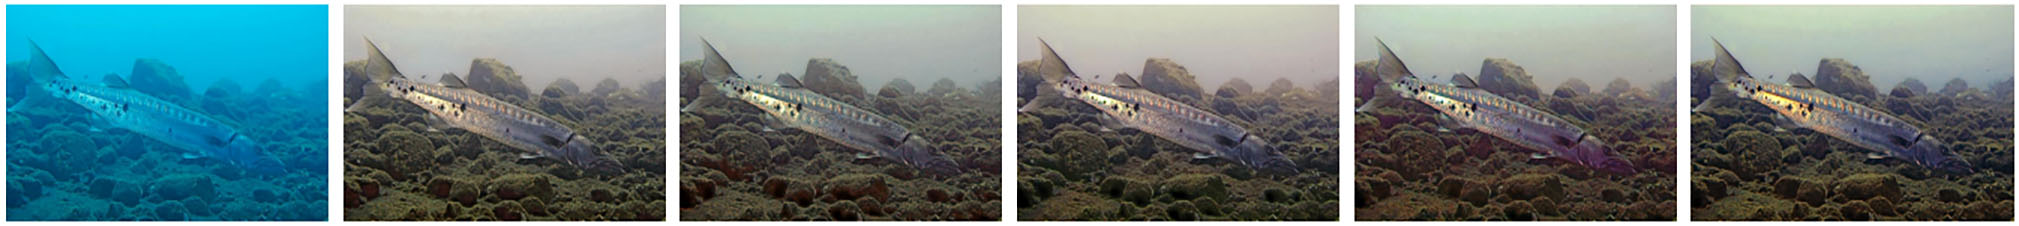
\includegraphics[width=1\textwidth]{FSpiralGAN_frontiers/onepicture/abalation_loop300.jpg}
\end{center}
$~~~~~~~~~~~~~$\textbf{A}$~~~~~~~~~~~~~~~~~~~~~~~~~$\textbf{B}$~~~~~~~~~~~~~~~~~~~~~~~~~$\textbf{C}$~~~~~~~~~~~~~~~~~~~~~~~~~~$\textbf{D}$~~~~~~~~~~~~~~~~~~~~~~~~~$\textbf{E}$~~~~~~~~~~~~~~~~~~~~~~~~~~$\textbf{F}
 \caption{Visual results with different spiral loops. From left to right, (\textbf{A}) shows the raw underwater images, and (\textbf{B-F}) are the results of second loops, fourth loops, sixth loops, eighth loops and tenth loops (Ours), respectively. \label{fig:abalation-loop}}
\end{figure}

\begin{figure}[htbp]
\begin{center}
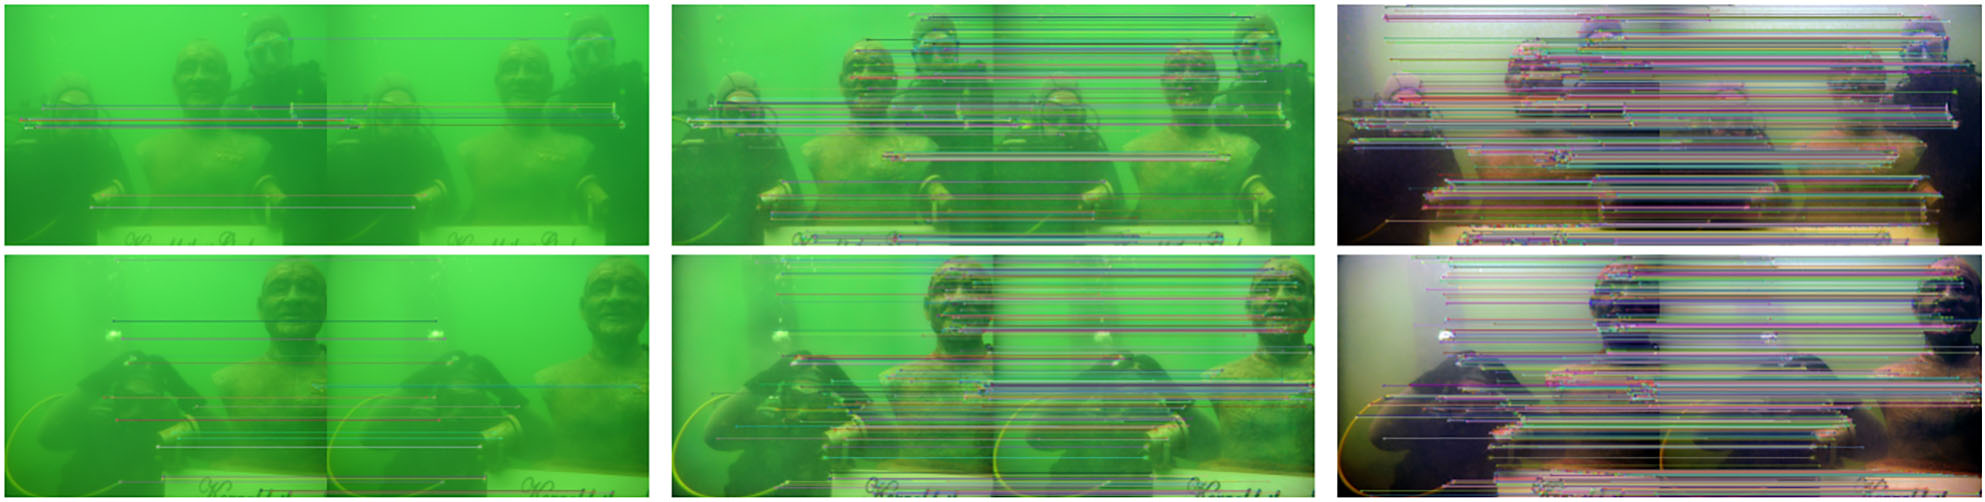
\includegraphics[width=0.8\textwidth]{FSpiralGAN_frontiers/onepicture/SIFT300.jpg}
\end{center}
$~~~~~~~~~~~~~~~~~~~~~~~~~~~~~~~~~~~~~~$\textbf{A}$~~~~~~~~~~~~~~~~~~~~~~~~~~~~~~~~~~~~~~~~~~$\textbf{B}$~~~~~~~~~~~~~~~~~~~~~~~~~~~~~~~~~~~~~~~~~~$\textbf{C}
 \caption{The visual results of keypoint matching. From left to right, (\textbf{A}) shows raw underwater images, and (\textbf{B-C}) are the results of CLAHE and the proposed model, respectively. \label{fig:comparison-SIFT}}
\end{figure}

\begin{table}[htbp]\normalsize
\centering
\setlength\tabcolsep{10pt}
\caption{The results of keypoint matching.}
\begin{tabular}{c|ccc}
\hline  
Method&Original&CLAHE&Ours\\
\hline 
picture1&29&261&\textbf{1193}\\
\hline 
picture2&35&308&\textbf{854}\\
\hline 
\end{tabular}
\label{tbl:comparison-SIFT}
\end{table}

\begin{figure}[htbp]
\begin{center}
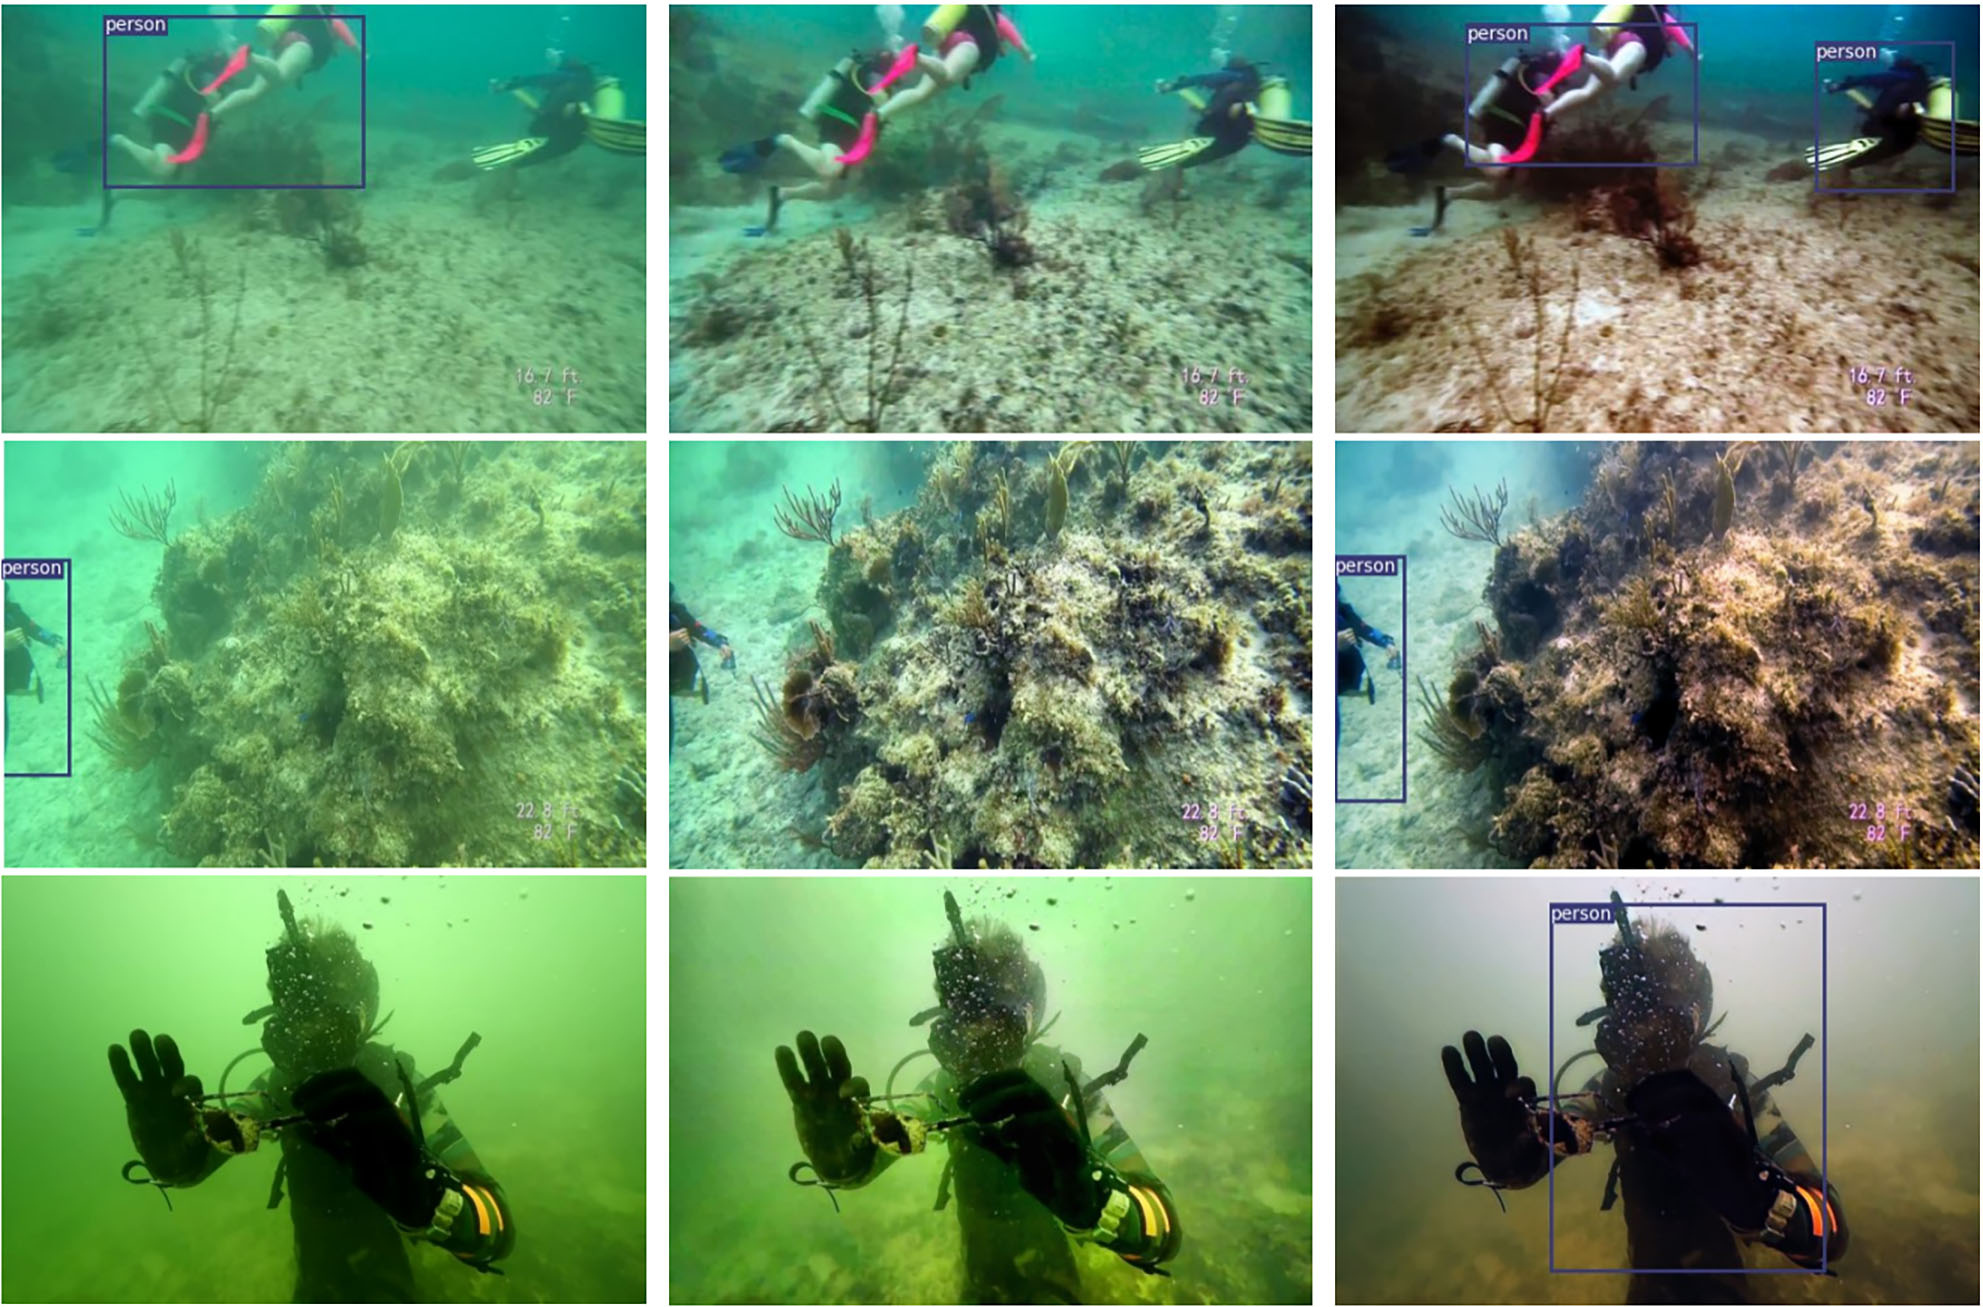
\includegraphics[width=0.45\textwidth]{FSpiralGAN_frontiers/onepicture/object_detection300.jpg}
\end{center}
$~~~~~~~~~~~~~~~~~~~~~~~~~~~~~~~~~~~~~~~~~~~~~~~~~~~~~~~~~$\textbf{A}$~~~~~~~~~~~~~~~~~~~~~~~$\textbf{B}$~~~~~~~~~~~~~~~~~~~~~$\textbf{C}
 \caption{Visual results of object detection. From left to right, (\textbf{A}) shows the raw underwater images, and (\textbf{B-C}) are the results of CLAHE and the proposed model, respectively. \label{fig:comparison-object detection}}
\end{figure}

\begin{figure}[htbp]
\begin{center}
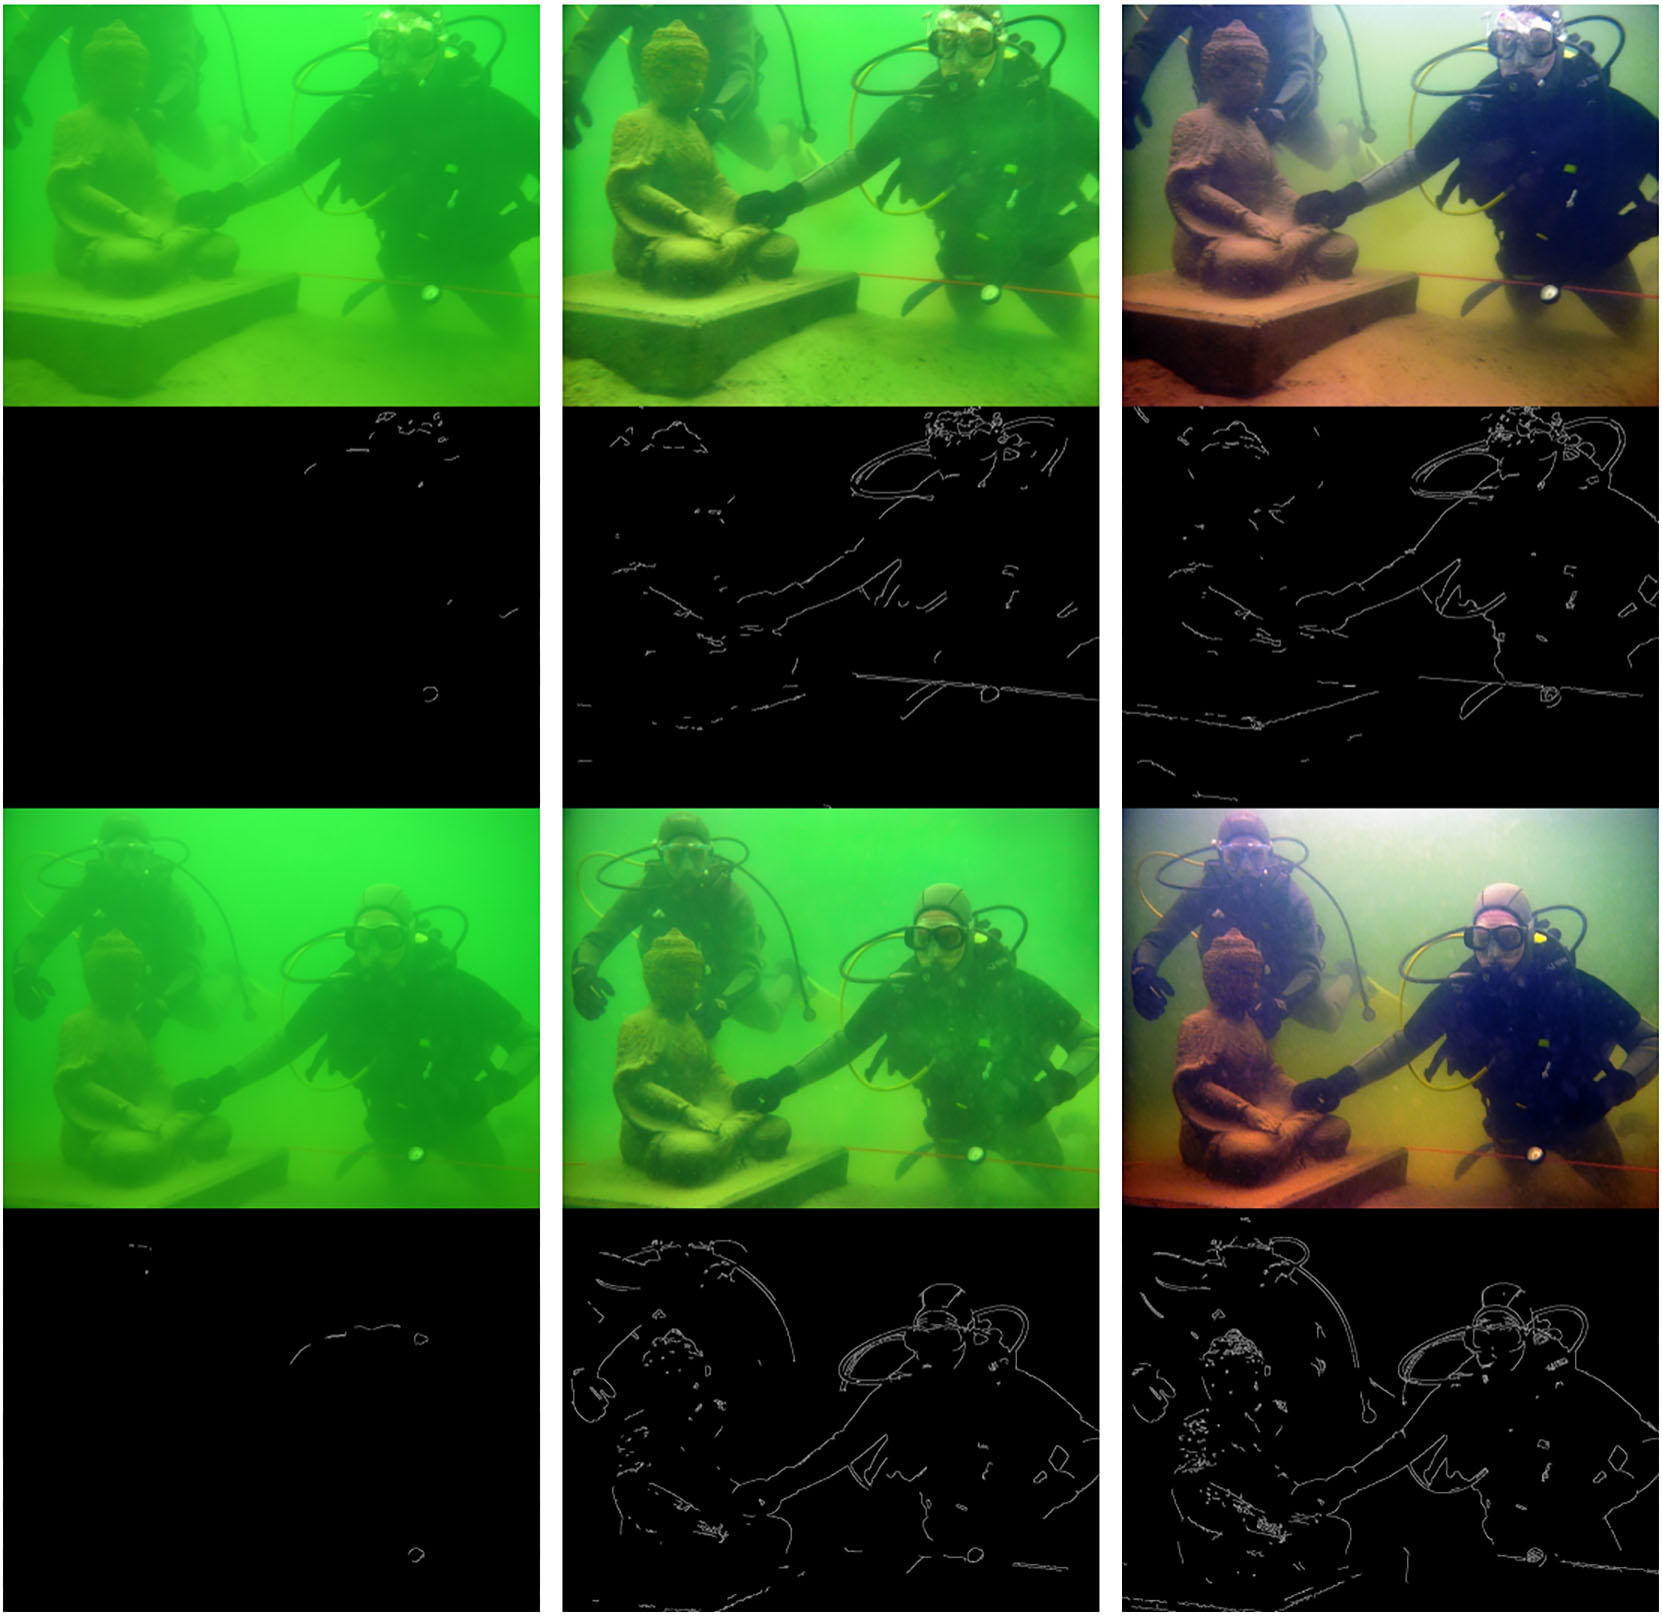
\includegraphics[width=0.45\textwidth]{FSpiralGAN_frontiers/onepicture/canny300.jpg}
\end{center}
$~~~~~~~~~~~~~~~~~~~~~~~~~~~~~~~~~~~~~~~~~~~~~~~~~~~~~~~~~$\textbf{A}$~~~~~~~~~~~~~~~~~~~~~~~$\textbf{B}$~~~~~~~~~~~~~~~~~~~~~~~$\textbf{C}
 \caption{The visual results of Canny edge detection. From left to right, (\textbf{A}) shows the raw underwater images, and (\textbf{B-C}) are the results of CLAHE and the proposed model, respectively. \label{fig:comparison-canny}}
\end{figure}

\end{document}
